%%
%% Template chap2.tex
%%

\chapter{Experiment 1: Learning with Random Sampling}
\label{cha:expt1}

Before we can get to the main investigation of Thompson sampling in Chapter \ref{cha:expt2}, we
need to first prepare the datasets and study them in the standard setting of supervised machine
learning. This, in turn, will help us design the protocol of the active learning experiment. In
particular, we start by doing feature selection (Section \ref{sec:prep}) and compare three sets of
extinction vectors (Section \ref{sub:extinction}) with the SDSS dataset. We then optimise the
hyperparameters of our classifiers (Section \ref{sub:hyper}) and obtain learning curves of both the
SDSS and VST ATLAS datasets (Section \ref{sub:lc}). Finally, the best-performing classifier is used
to predict the unknown class proportion of the 800 unlabelled objects in the SDSS (Section
\ref{sub:prop}).


\section{Preparation of Data}
\label{sec:prep}

The VST ATLAS dataset has been specifically prepared for us by Christian Wolf from the ANU Research
School of Astronomy \& Astrophysics, so there is no need to do any cleaning or feature selection.
The SDSS dataset, on the other hand, was extracted from the Sloan SkyServer. Appendix
\ref{cha:datasets} contains instructions on how to replicate the data, including relevant SQL
queries. In particular, we extract two sets of data. For the labelled objects, we only include
those that have a clean spectrum and hence a reliable spectroscopic label. We do not impose any
limit on how faint an object can be, but we do exclude those with a photometric error greater than
3 mag (i.e. 3 orders of magnitudes in brightness). This is deliberate since it allows us to
investigate how well our classifiers can deal with noisy data. Given the constraints, the resulting
labelled set contains 2.8 million objects. Finally, the second set of SDSS data contains
photometric measurements of all 800 million objects in the database. No constraints were applied to
this set.

Originally, each object has 5 PSF and 5 Petrosian magnitudes. As we discussed in Section
\ref{sub:colours} however, it is better to take the differences and obtain the colours. By
convention, we calculate the $u-g$, $u-r$, $r-i$, and $i-z$ colours. In addition, we keep one
apparent magnitude in the set of features. The magnitude in the r-band is chosen since it lets the
the greatest fraction of light through the filter. This, hopefully, would give us a high
signal-to-noise ratio. Although it has been not been rigorously verified, this combination of four
colours and one magnitude has been found to produce good results by astronomers in the past [Wolf,
pers. comm.]. In the end, we end up with 11 features:
\begin{itemize}
	\item Four PSF and four Petrosian colours ($u-g$, $u-r$, $r-i$, $i-z$).
    \item The r-band PSF and the r-band Petrosian magnitudes.
	\item The r-band Petrosian radius.
\end{itemize}
For a quick visualisation of these features, we make a scatter plot in Figure
\ref{fig:sdss_pca_all} of the first two principal components. Although we can clearly see clusters
of stars, quasars, and galaxies, there is also enough  overlap between classes, especially
between stars and quasars, to make the problem interesting.

Finally, we scale all the features in both datasets to have a zero mean and a unit variance.
Although this has little effect in random forests, feature scaling is important for logistic
regression and SVMs.

\begin{figure}[tbp]
	\centering
	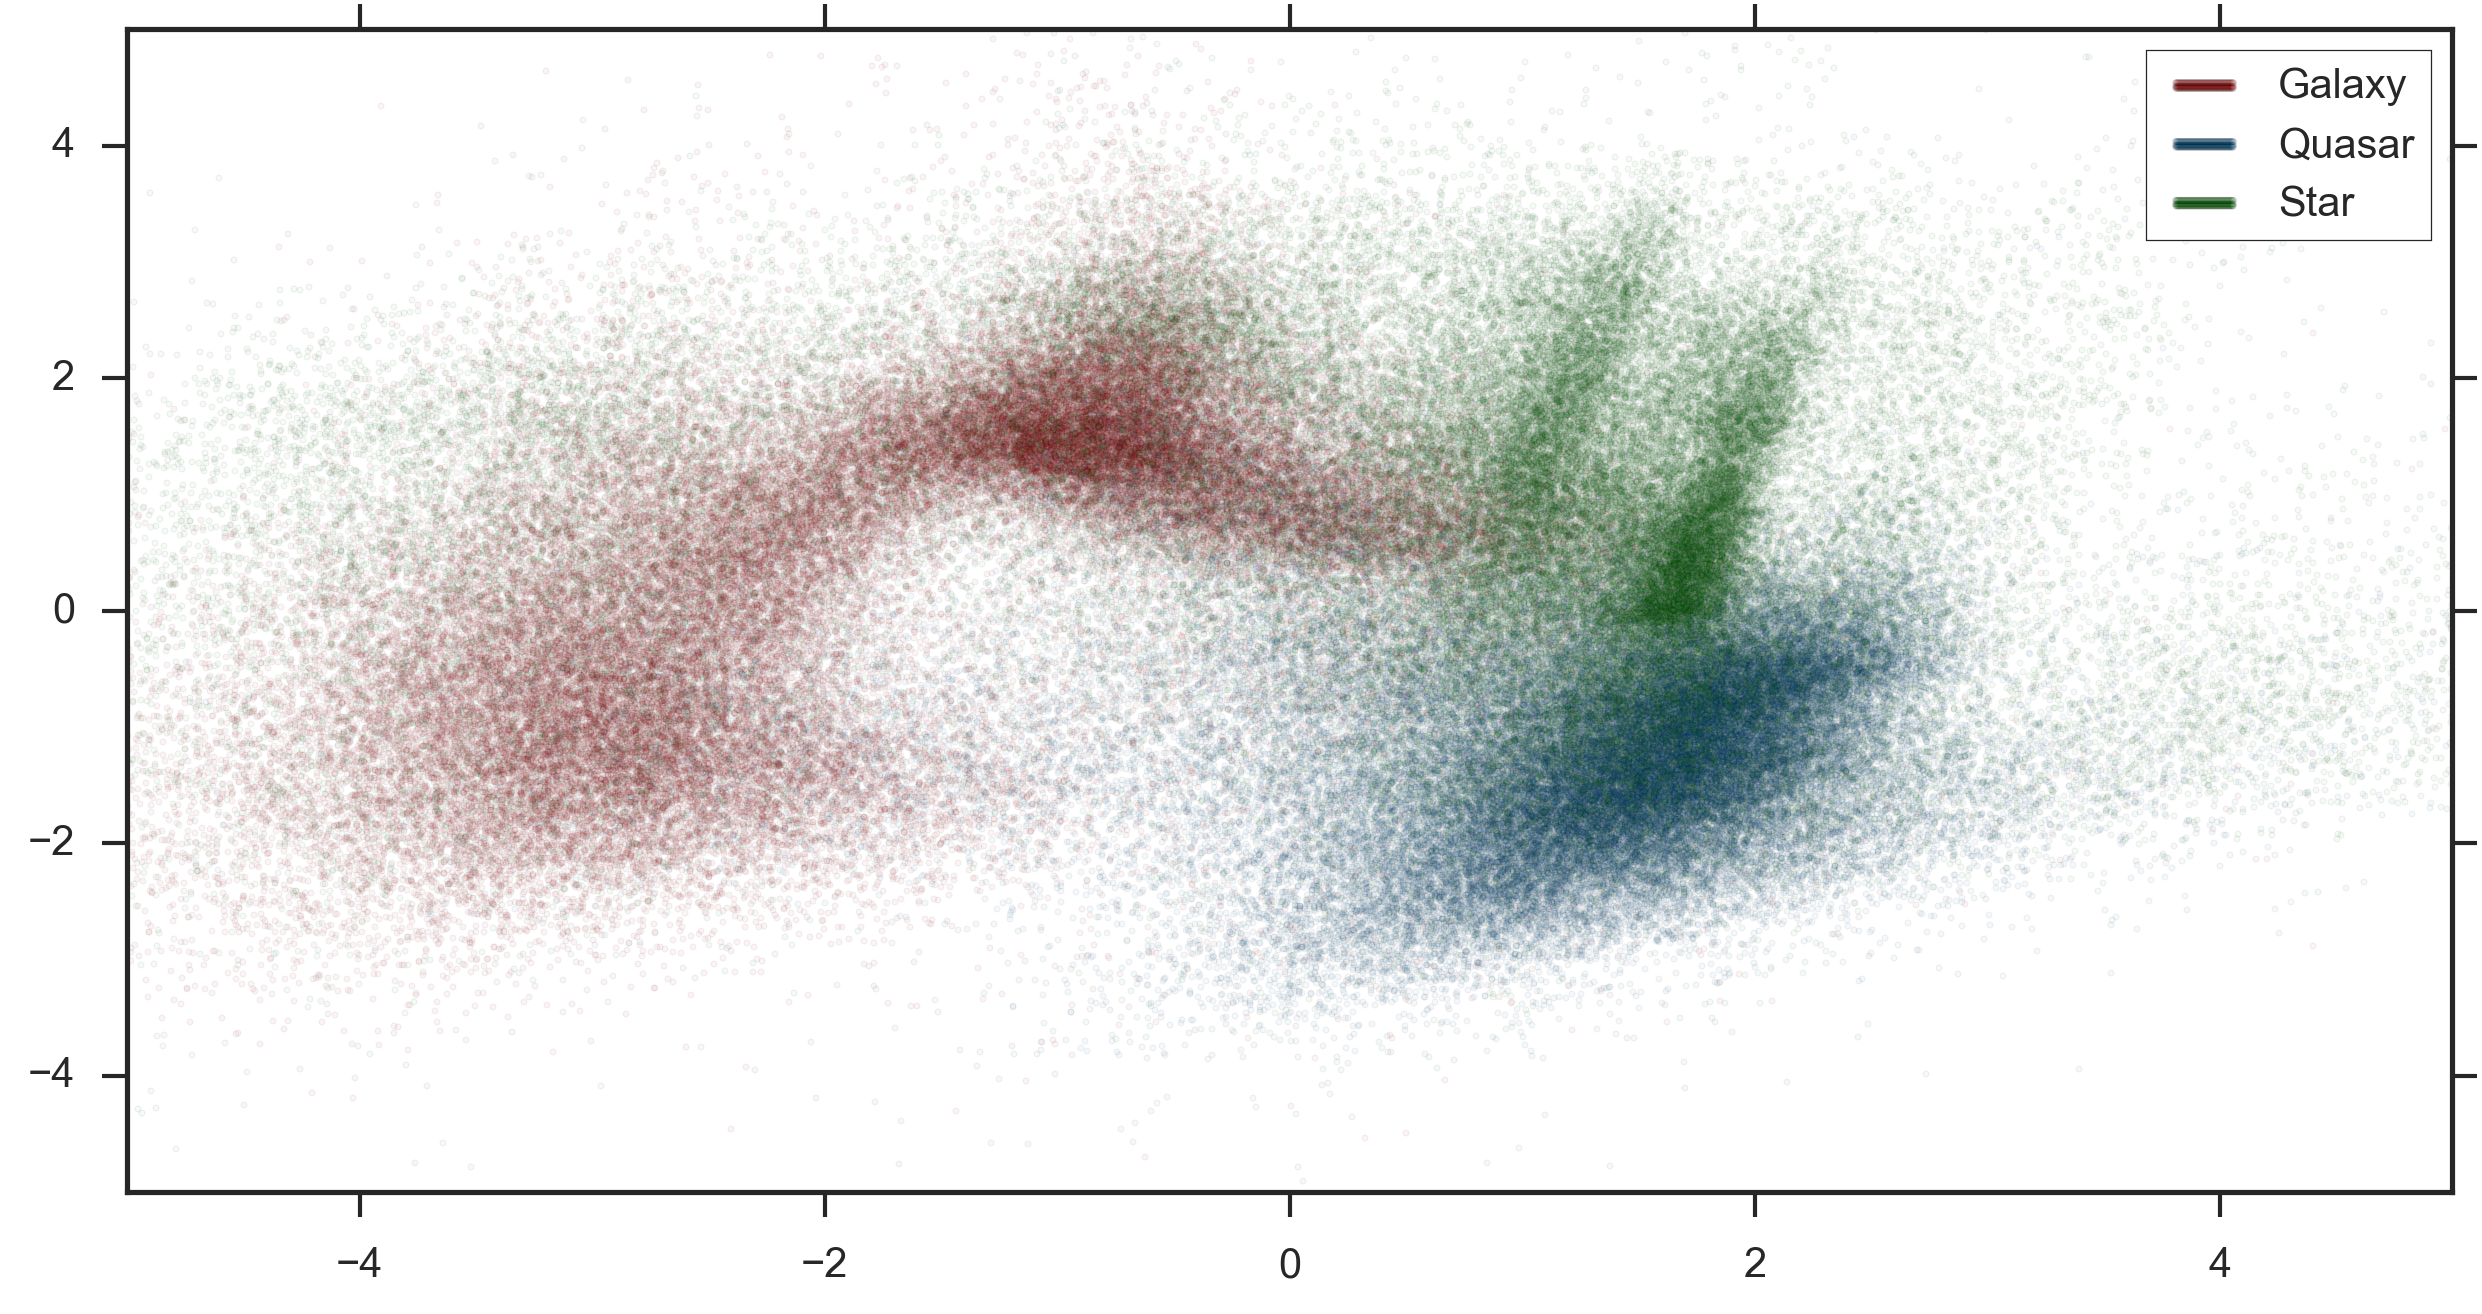
\includegraphics[width=\textwidth]{figures/4_expt1/sdss_pca_all}
	\caption[First two principal components of the SDSS dataset]{We use principal
		component analysis (PCA) to reduce the 11 features of the SDSS dataset down
		to two dimensions. This allows us to do a quick visual scan and see how
		separable the three classes are.}
	\label{fig:sdss_pca_all}
\end{figure}


\section{Experimental Protocol}
\label{sec:protocol1}

This experiment consists of three parts. We first compare three sets of reddening correction.
We then examine the performance of various classifiers with random sampling. Finally
we pick the best classifier and use it to predict the unknown proportions in the unlabelled
set.

\subsection{Reddening Correction}
\label{sub:red}

To compare the three extinction vectors (SDF98, SF11, and W14), we first split the labelled pool
into a balanced training set of size 600,000 and a balanced test set of size 300,000. We then apply
each correction to the measurements and train a random forest of 300 decision trees. A random
forest is chosen due to its speed of execution. Finally the balanced posterior accuracy on the test
set allows us to decide on the best performing reddening correction set. This set will be applied
in all subsequent experiments.

\subsection{Comparing Classifiers}
\label{sub:compare}

Next we would like to compare the performance of four classifiers: random forests, logistic
regression, linear SVMs, and SVMs with an RBF kernel. In the random forest,
we again build 300 trees and the
Gini impurity is used to measure the quality of a split. With the other classifiers,
there
are a few hyperparameters that require tuning before training, including the degree of the polynomial
transformation of the original features. To find the optimal values,
we conduct a search in the parameter space with logarithmic steps. For each combination,
we do a five-fold cross validation with a training and test size of 300 each. We then plot
the results on a heat map.

Once the hyperparameters are optimised, we compare the performance of the classifiers by looking at
their learning curves. The VST ATLAS data is fairly small, so we can use all of the examples. Since
using all of the SDSS labelled examples would take too long on some classifiers like logistic
regression, we stop at 300,000 examples. To smooth out the curve, we do a stratified shuffle split
with 5 iterations, and then take an average of the results.

Since we would like to use as much data as possible, no attempt is made to balance the classes.
Instead we give to the classifiers a weight vector that is proportional to the inverse
of the class frequencies. This means that rare objects like white dwarfs are given more
weight during training. In addition, we use the posterior balance accuracy rate to remove
any bias toward the dominant class.

Finally since we have 800 million unlabelled objects in the SDSS, we pick the best performing
classifier and predict the class proportion on the unlabelled data. Information from the confusion
matrix is used to correct for the potential misclassification.

\section{Results and Discussion}
\label{sec:results1}

\subsection{Comparison of Reddening Correction Sets}
\label{sub:extinction}

Figure \ref{fig:reddeningviolin} on page \pageref{fig:reddeningviolin} shows the violin plot of the
posterior balanced accuracy on the test set when we apply each of the three extinction vectors to
the measurements. Appendix \ref{cha:supp} contains more detailed results. Overall, the results are
quite uninteresting since no statistical differences can be found between the three sets. In fact,
even if we do not apply any correction, the accuracy rate still remains unchanged.

This could be because in the SDSS did not survey many objects in the Milky Way band, the region in
which there is the most dust extinction. Indeed, if we look back at the reddening map in Figure
\ref{fig:reddening}, although the extinction amount does vary through the field, such variation is
probably fairly small and random forests, after all, are quite robust to noise. In any case, for
good measure, we shall correct all photometric measurements for dust extinction using the latest
W14 set. Other projects like SkyMapper will survey regions closer to the Milky Way band and thus
future work using its data might be able to provide more conclusive evidence of which of the three
extinction vectors provides the biggest improvement to the accuracy rate.

\begin{figure}[tbp]
	\centering
	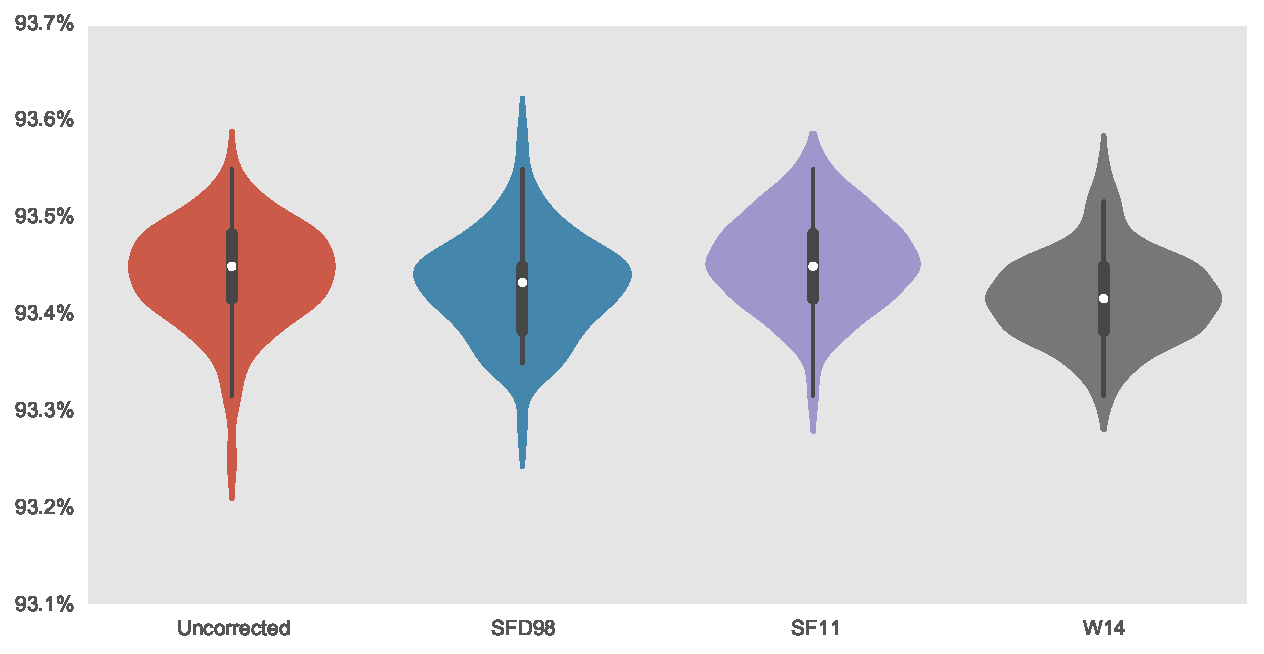
\includegraphics[width=\textwidth]{figures/4_expt1/violin_reddening_correction}
	\caption[Accuracy rates with three extinction vectors]{Violin plots
		showing the posterior distribution of the balanced accuracy rates: Inside each
		violin is a boxplot, where the white dot represents the mean. Given the overlapping,
        there is no statistical difference between the four extinction vectors.}
	\label{fig:reddeningviolin}
\end{figure}

\subsection{Hyperparameter Optimisations}
\label{sub:hyper}

The next three pages contain heat maps of the cross-validation accuracy rate
for many different combinations of hyperparameters. For readability, we provide detailed
reasoning under each figure of how we choose the optimal values of the parameters.
Below is a summary of our decisions:
\begin{itemize}
	\item \textbf{Logistic Regression}: We do first a degree 2 polynomial transformation of both
	the SDSS and the VST ATLAS features. For the classifier, we use the one-vs-rest
	strategy and an L1-norm for the penalisation, thus giving us sparse solutions. The inverse
	regularisation term $C$ is 1 in SDSS and 100 in VST ATLAS.
    
	\item \textbf{Linear SVM}: For the SDSS data, we do a degree 2 polynomial transformation
	and our classifier uses the one-vs-rest strategy with the squared hinge loss function
	and, an L1-norm, and $C=0.1$. For the VST ATLAS data, we simply
    use the Crammer-Singer approach with $C = 1,000$.
	\item \textbf{SVM with RBF Kernel}: The optimal hyperparameter values for the SDSS data are
	$\gamma = 0.01$ and $C = 1,000$. For the VST ATLAS data, they are $\gamma = 0.001$ and
	$C = 1,000,000$.
\end{itemize}

\begin{figure}[p]
	\centering
	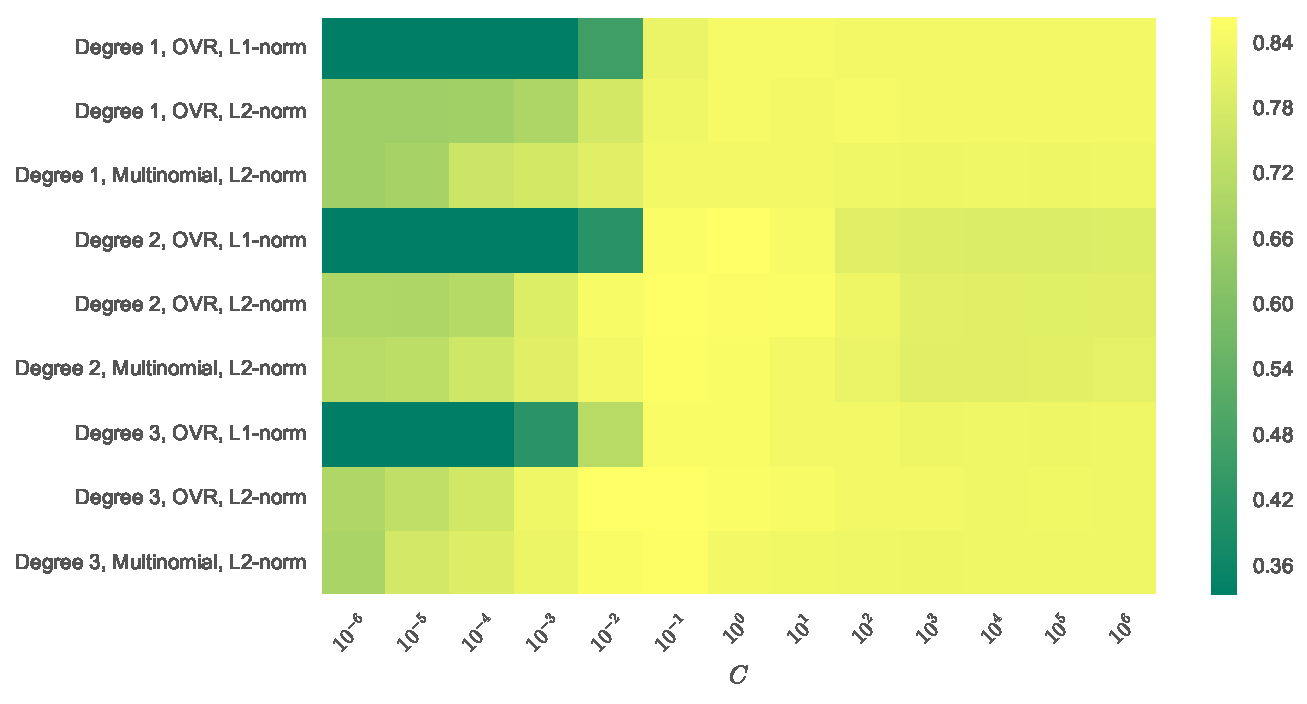
\includegraphics[width=\textwidth]{figures/4_expt1/sdss_grid_logistic}
	\caption[Heat map of logistic regression's CV accuracy in SDSS]{
		Heat map of linear logistic regression's cross-validation accuracy in the SDSS dataset:
		The best-performing combination involves doing a degree 3 polynomial transformation
		of the features. In practice, this would make it too slow to run subsequent experiments.
		Thus we sacrifice a bit of accuracy and pick the optimal parameters that
		involve only a degree 2 polynomial transformation. In particular, we set the inverse regularisation
		term $C$ to be 1 and use the one-vs-rest strategy with L1-norm.}
	\label{fig:sdss_grid_logistic}
\end{figure}

\begin{figure}[p]
	\centering
	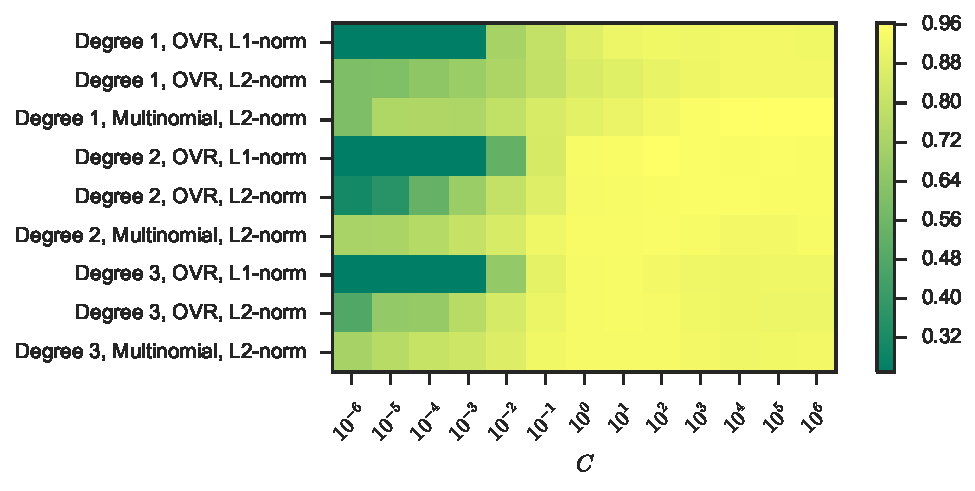
\includegraphics[width=\textwidth]{figures/4_expt1/vstatlas_grid_logistic}
	\caption[Heat map of logistic regression's CV accuracy in VST ATLAS]{
		Heat map of logistic regression's cross-validation accuracy in the VST ATLAS dataset:
		The optimal combination involves using multinomial logistic regression. This
		might seem like a good choice since we get true probability estimates. However
		it turns out that the scikit-learn implementation of multinomial regression
		gives unstable probabilities. Thus we resort to the next best combination,
		where we use one-vs-rest, a degree 2 polynomial transformation of the features, and $C = 100$. }
	\label{fig:vstatlas_grid_logistic}
\end{figure}

\begin{figure}[p]
	\centering
	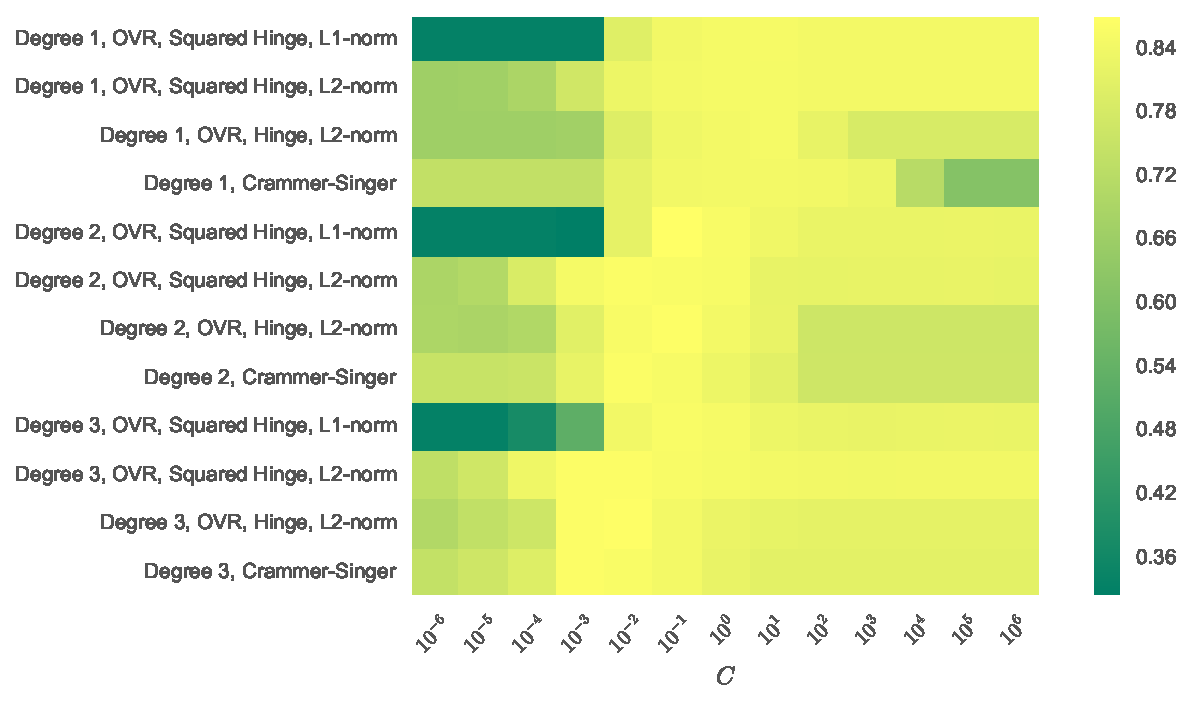
\includegraphics[width=\textwidth]{figures/4_expt1/sdss_grid_poly}
	\caption[Heat map of linear SVM's CV accuracy in SDSS]{
		Heat map of linear SVM's cross-validation accuracy in the SDSS dataset:
		Like Figure \ref{fig:sdss_grid_logistic}, the optimal
		combination involves a degree 3 polynomial transformation of the features.
		Due to constraints on
		processing power, we shall instead pick the next best alternative, which involves
		a degree 2 transformation, the one-vs-rest strategy, the squared hinge loss function,
		and the L1-norm for the penalisation.}
	\label{fig:sdss_grid_poly}
\end{figure}

\begin{figure}[p]
	\centering
	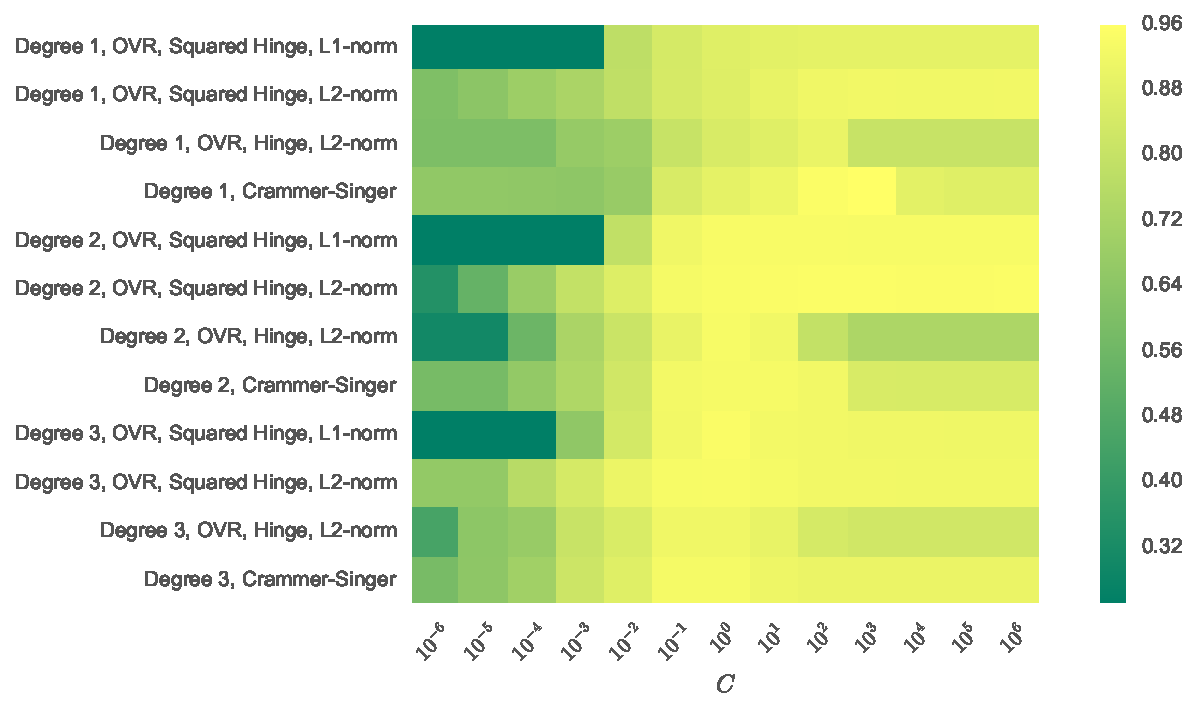
\includegraphics[width=\textwidth]{figures/4_expt1/vstatlas_grid_poly}
	\caption[Heat map of linear SVM's CV accuracy in VST ATLAS]{
		Heat map of linear SVM's cross-validation accuracy in the VST ATLAS dataset:
		Interestingly, the optimal combination does not require any polynomial
		transformation of the features, and instead of the usual one-vs-rest strategy,
		we use the Crammer-Singer method
		with $C = 1000$ gives the best result. In theory, the Crammer-Singer approach
		can give us true probability estimates, however this has not been implemented
		in scikit-learn.}
	\label{fig:vstatlas_grid_poly}
\end{figure}

\begin{figure}[p]
	\centering
	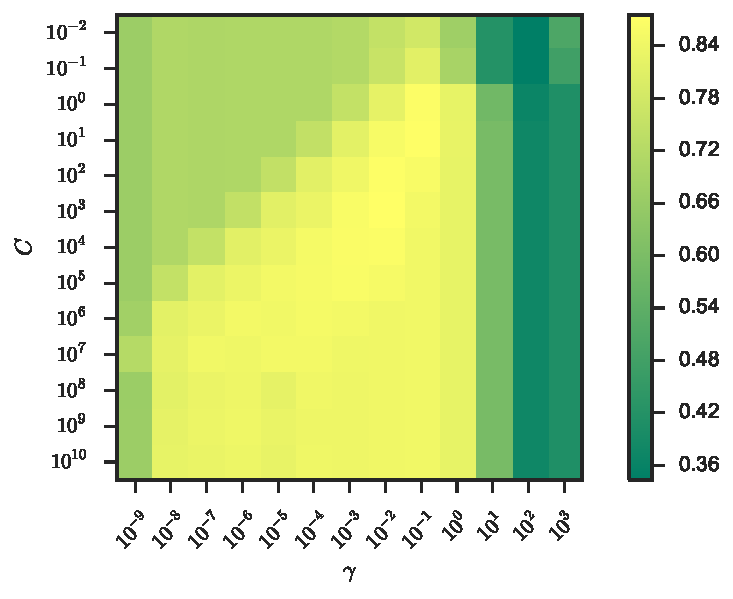
\includegraphics[width=0.7\textwidth]{figures/4_expt1/sdss_grid_rbf}
	\caption[Heat map of RBF SVM's CV accuracy in SDSS]{
		Heat map of RBF SVM's cross-validation accuracy in the SDSS dataset:
		Here the optimal values for the hyperparameters are $\gamma=0.01$
		and $c = 1,000$, giving an accuracy of around $88\%$.}
	\label{fig:sdss_grid_rbf}
\end{figure}

\begin{figure}[p]
	\centering
	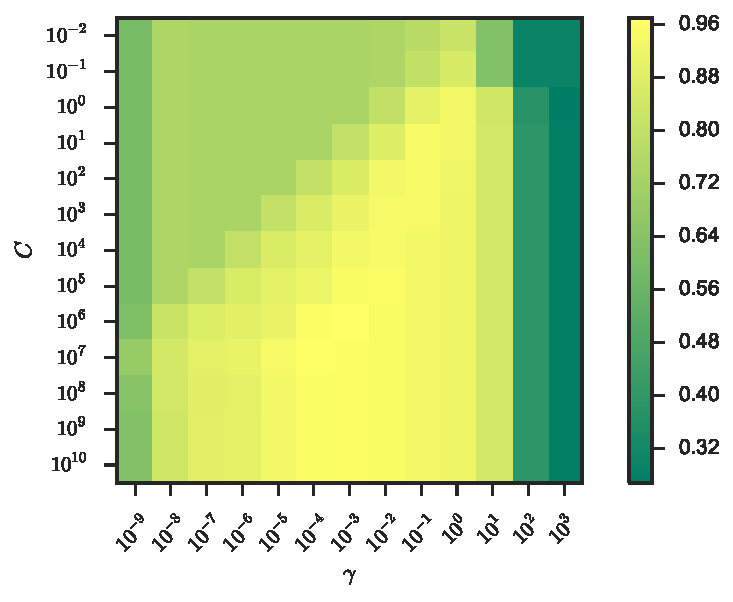
\includegraphics[width=0.7\textwidth]{figures/4_expt1/vstatlas_grid_rbf}
	\caption[Heat map of RBF SVM's CV accuracy in VST ATLAS]{
		Heat map of RBF SVM's cross-validation accuracy in the VST ATLAS dataset:
		The optimal values are $\gamma=0.001$ and $C = 1,000,000$, giving us an accuracy
		of $97\%$. Observe that
		with a large value of $C$, we would need more support vectors during training
		and hence the the model will be somewhat slower at prediction.}
	\label{fig:vstatlas_grid_rbf}
\end{figure}


\subsection{Learning Curves with Random Sampling}
\label{sub:lc}

Now that we have tuned the hyperparameters, we are ready to compare the classifiers. Figure
\ref{fig:learning_curves} shows the average learning curves of the two datasets. Overall the two
best performers are random forests and SVMs with an RBF kernel. The VST ATLAS data appears to be
very clean, with highest achievable balanced accuracy rate of 99\%. Logistic regression with a
degree 2 polynomial transformation is the slowest algorithm, surprising even slower than RBF SVMs
(in theory, it should be the other way around). This could simply be due to the very efficient
kernel approximation implemented in scikit-learn.

\begin{figure}[tbp]
	\centering
	\begin{subfigure}{.5\textwidth}
		\centering
		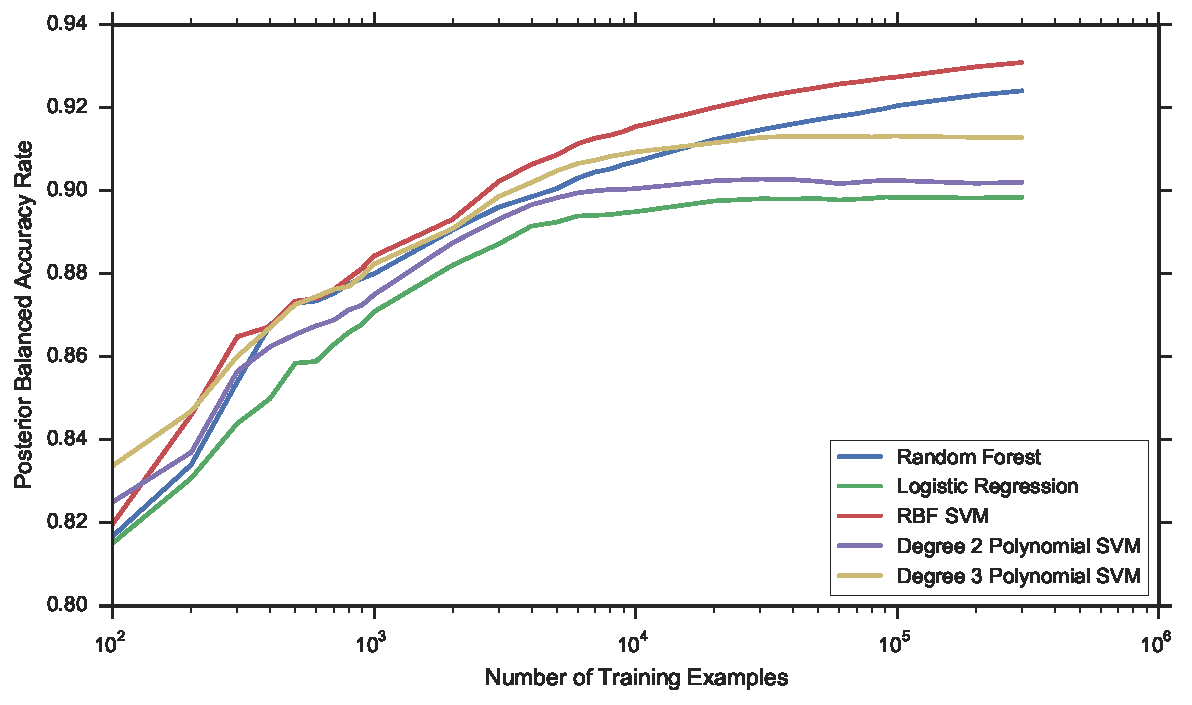
\includegraphics[width=0.99\textwidth]{figures/4_expt1/sdss_learning_curves}
		\caption{With SDSS data}
		\label{fig:sdss_learning_curves}
	\end{subfigure}%
	\begin{subfigure}{.5\textwidth}
		\centering
		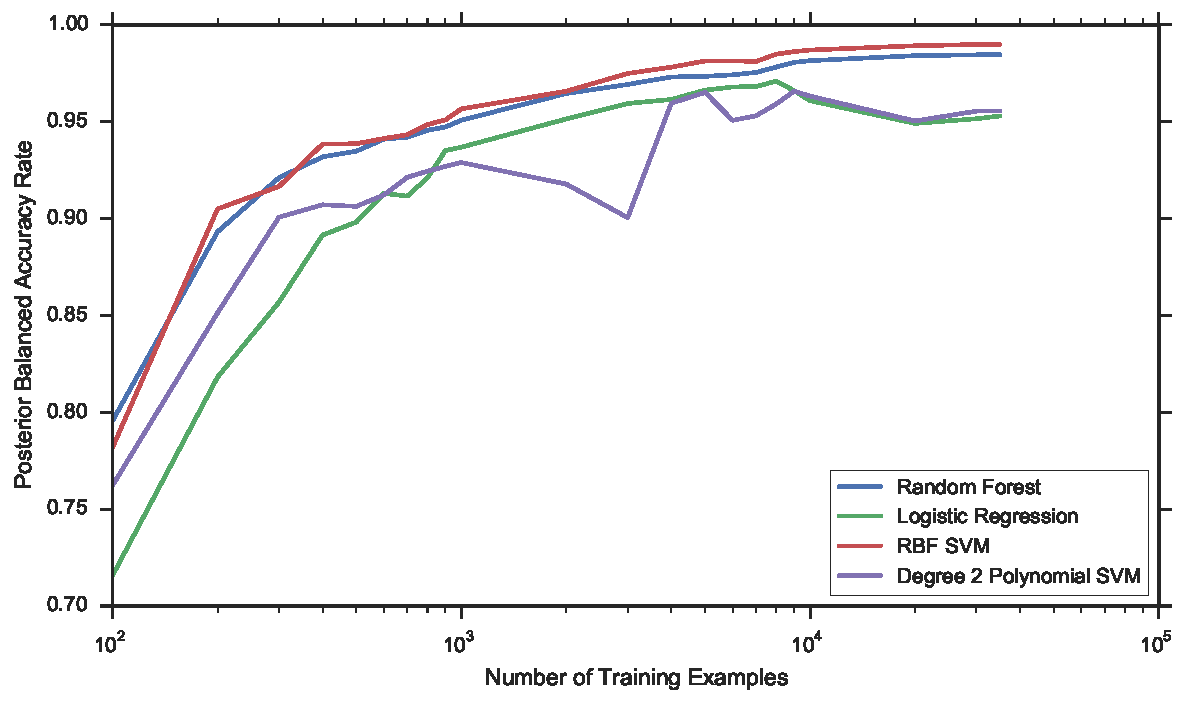
\includegraphics[width=0.99\linewidth]{figures/4_expt1/vstatlas_learning_curves}
		\caption{With VST ATLAS data}
		\label{fig:vstatlas_learning_curves}
	\end{subfigure}
	\caption[Learning curves with random sampling]{
		These are the average learning curves (of 5 trials) with random sampling.
		Note that we use a log scale for the x-axis since generally, it gets exponentially
		more difficult to improve the accuracy rate as the accuracy approaches 1.}
	\label{fig:learning_curves}
\end{figure}



\subsection{Class Proportion Estimation}
\label{sub:prop}

Let us now make some predictions on the unlabelled SDSS data. Although the RBF SVM is
the best-performing classifier, we nonetheless choose the random forest due to its fast
training time. We retrain the forest, now with a training set of size 837,000 and a test
set of size 300,000. Figure \ref{fig:confusion} shows the confusion matrix on the test set.
Observe that it is easiest to classify galaxies and the main difficulty is distinguishing
between stars and quasars.

There are exactly 794,014,031 objects in the entire database. Out of these, the random 
forest predicts that
	\begin{itemize}
		\item 357,910,241 (45.1\%) are galaxies
		\item 266,083,661 (33.5\%) are stars
		\item 170,020,129 (21.4\%) are quasars
	\end{itemize} 
Using information from the normalised confusion matrix, we might be able to correct
for the potential misclassification. For example, only 95.7\% of objects predicted as galaxies
are actually galaxies, while 0.5\% of objects predicted as stars are galaxies and 1.8\% of
objects predicted as quasars are galaxies. Let $Q_{ij}$ the entry in the $i$th
row and $j$th column of the normalised confusion matrix. Let $N_G$, $N_S$, and $N_Q$ be the
predicted number of galaxies, stars, and quasars, respectively; and let $N'_G$, $N'_S$, and $N'_Q$ be the actual numbers. Then the estimated actual number of galaxies,
stars, and quasars in the unlabelled pool are
	\begin{IEEEeqnarray*}{lCl}
		N'_G &=& N_G Q_{11} + N_S Q_{12} + N_Q Q_{13} = 376,281,067 \\
		N'_S &=& N_G Q_{21} + N_S Q_{22} + N_Q Q_{23} = 145,832,927 \\
		N'_Q &=& N_G Q_{31} + N_S Q_{32} + N_Q Q_{33} = 271,900,036
	\end{IEEEeqnarray*}
Thus after the correction, around 43.7\% of objects are galaxies, 34.5\% are stars, and 21.8\% are
quasars. Note however that even the full SDSS dataset is not a random sample of the sky. More
sophisticated methods are needed if we want to recover the true proportions of the random sky.


\begin{figure}[tbp]
	\centering
	\renewcommand\arraystretch{1.5}
	\setlength\tabcolsep{0pt}
	\begin{tabular}{c >{\bfseries}r @{\hspace{0.7em}}c @{\hspace{0.4em}}c @{\hspace{0.4em}}c}
		\multirow{13}{*}{\rotatebox{90}{\parbox{1.1cm}{\bfseries\raggedleft Actual}}} & 
		& \multicolumn{3}{c}{\bfseries Predicted} \\
		& & \bfseries Galaxy & \bfseries Star & \bfseries Quasar \\
		& Galaxy & \MyBox{97,608}{95.7\%} & \MyBox{500}{0.5\%} & \MyBox{1,892}{1.8\%} \\[2.4em]
		& Star & \MyBox{1,633}{1.6\%} & \MyBox{89,489}{95.4\%}  & \MyBox{8,878}{8.5\%} \\[2.4em]
		& Quasar & \MyBox{2,801}{2.7\%} & \MyBox{3,823}{4.1\%}  & \MyBox{93,376}{89.7\%}
	\end{tabular}
	\caption[Confusion matrix of the random forest with SDSS]{
		The confusion and the normalised confusion matrix of the random forest
		on the SDSS test set. For example, out of all the objects predicted as quasars, 8.5\%
		of them are actually stars. Out of all the objects predicted as stars, 4.1\% of them
		are actually quasars.}
	\label{fig:confusion}
\end{figure}

\begin{figure}[p]
	\centering
	\begin{subfigure}{\textwidth}
		\centering
		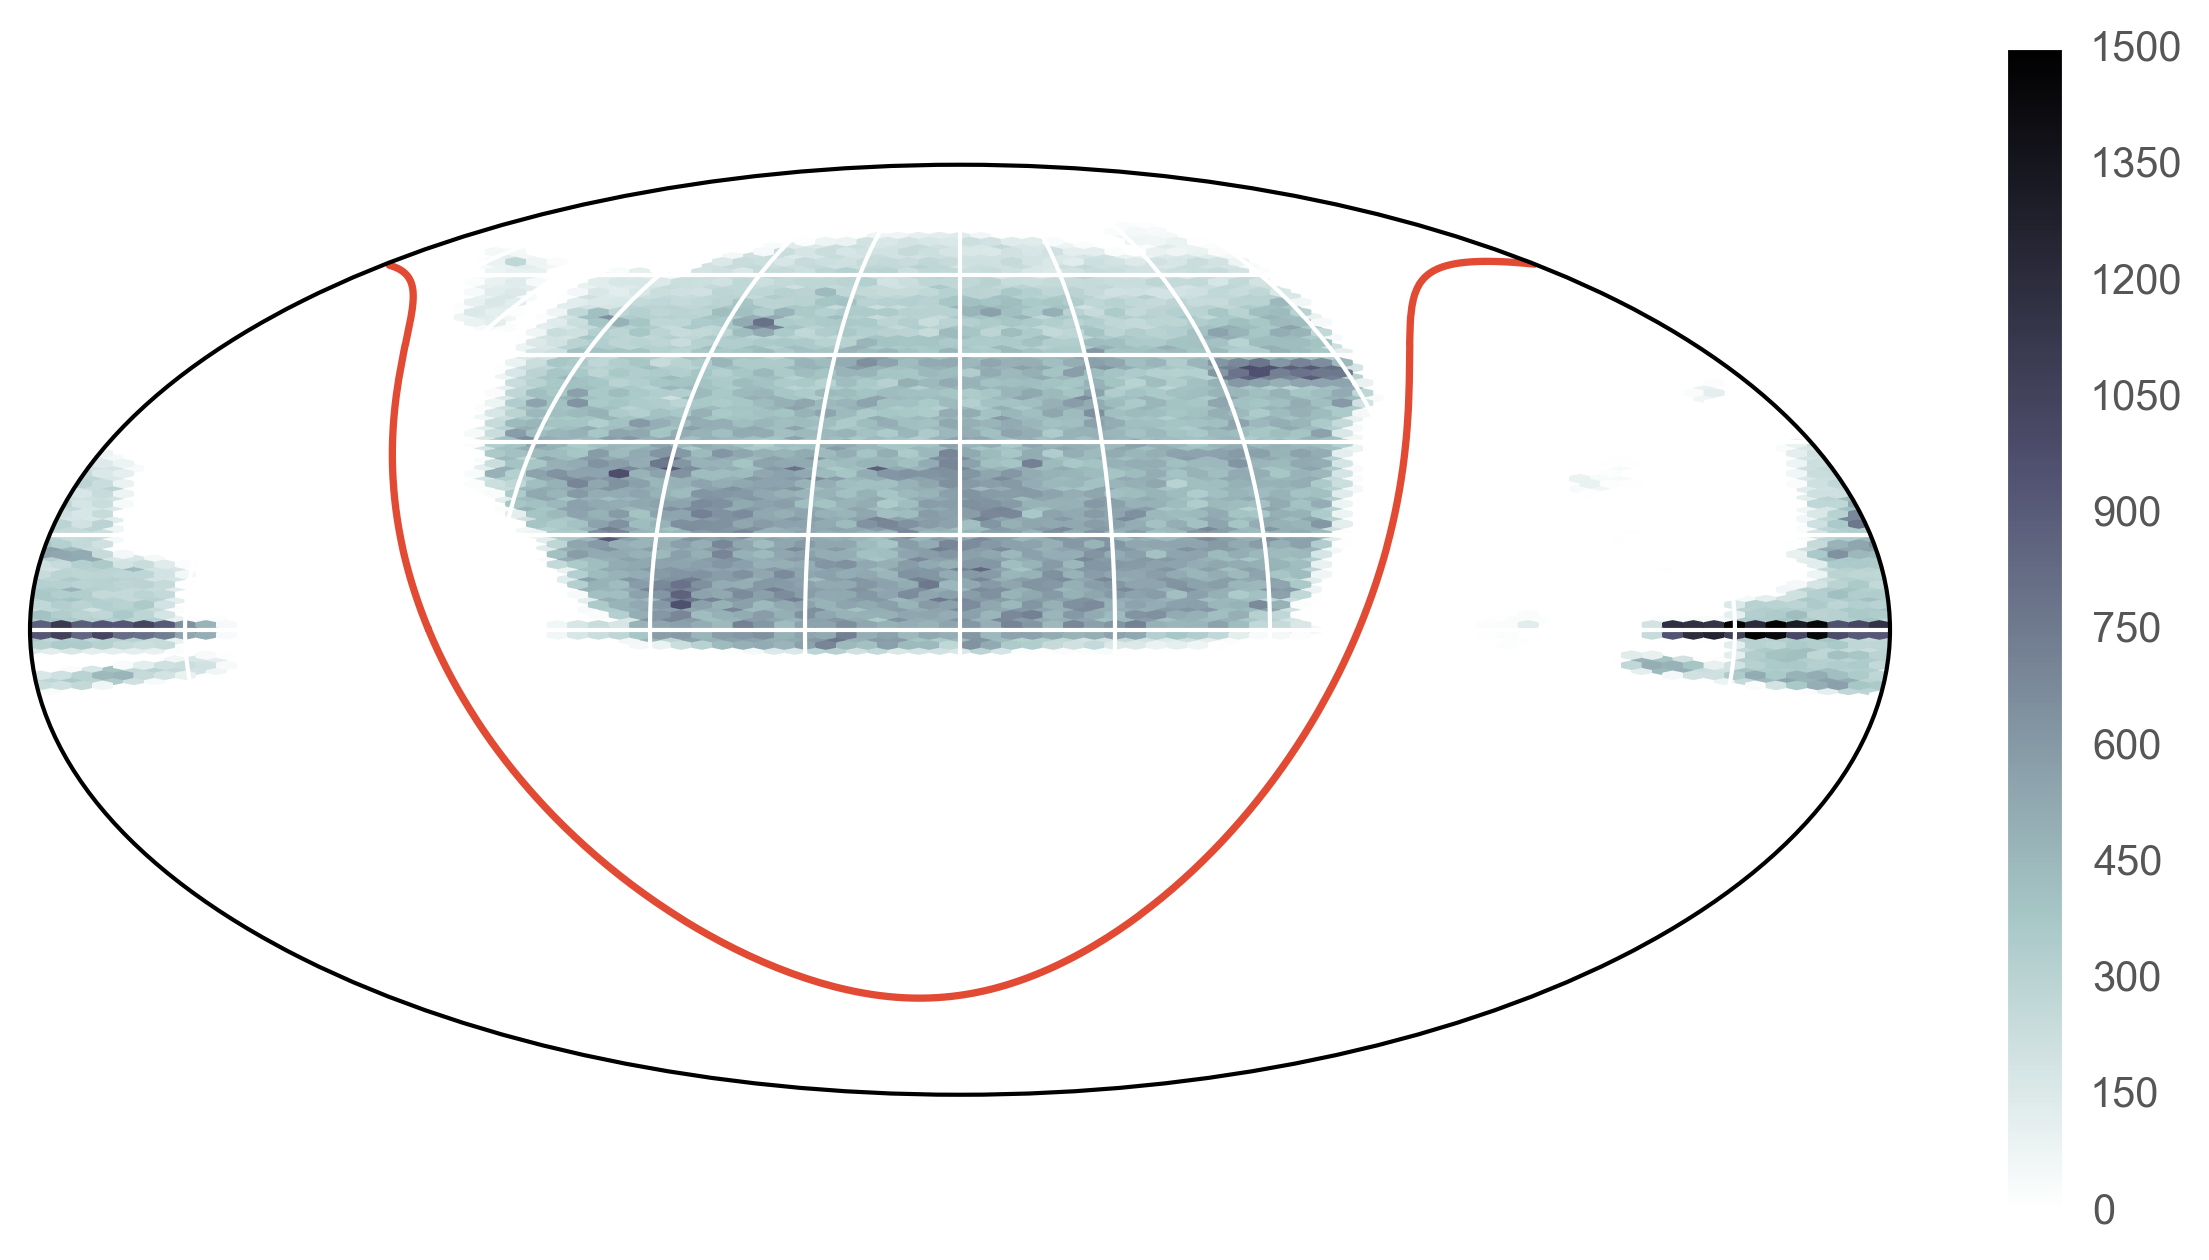
\includegraphics[width=0.73\textwidth]{figures/4_expt1/sdss_train_galaxies}
		\caption{The distribution of galaxies.}
		\label{fig:training_g}
	\end{subfigure}\\
	\begin{subfigure}{\textwidth}
		\centering
		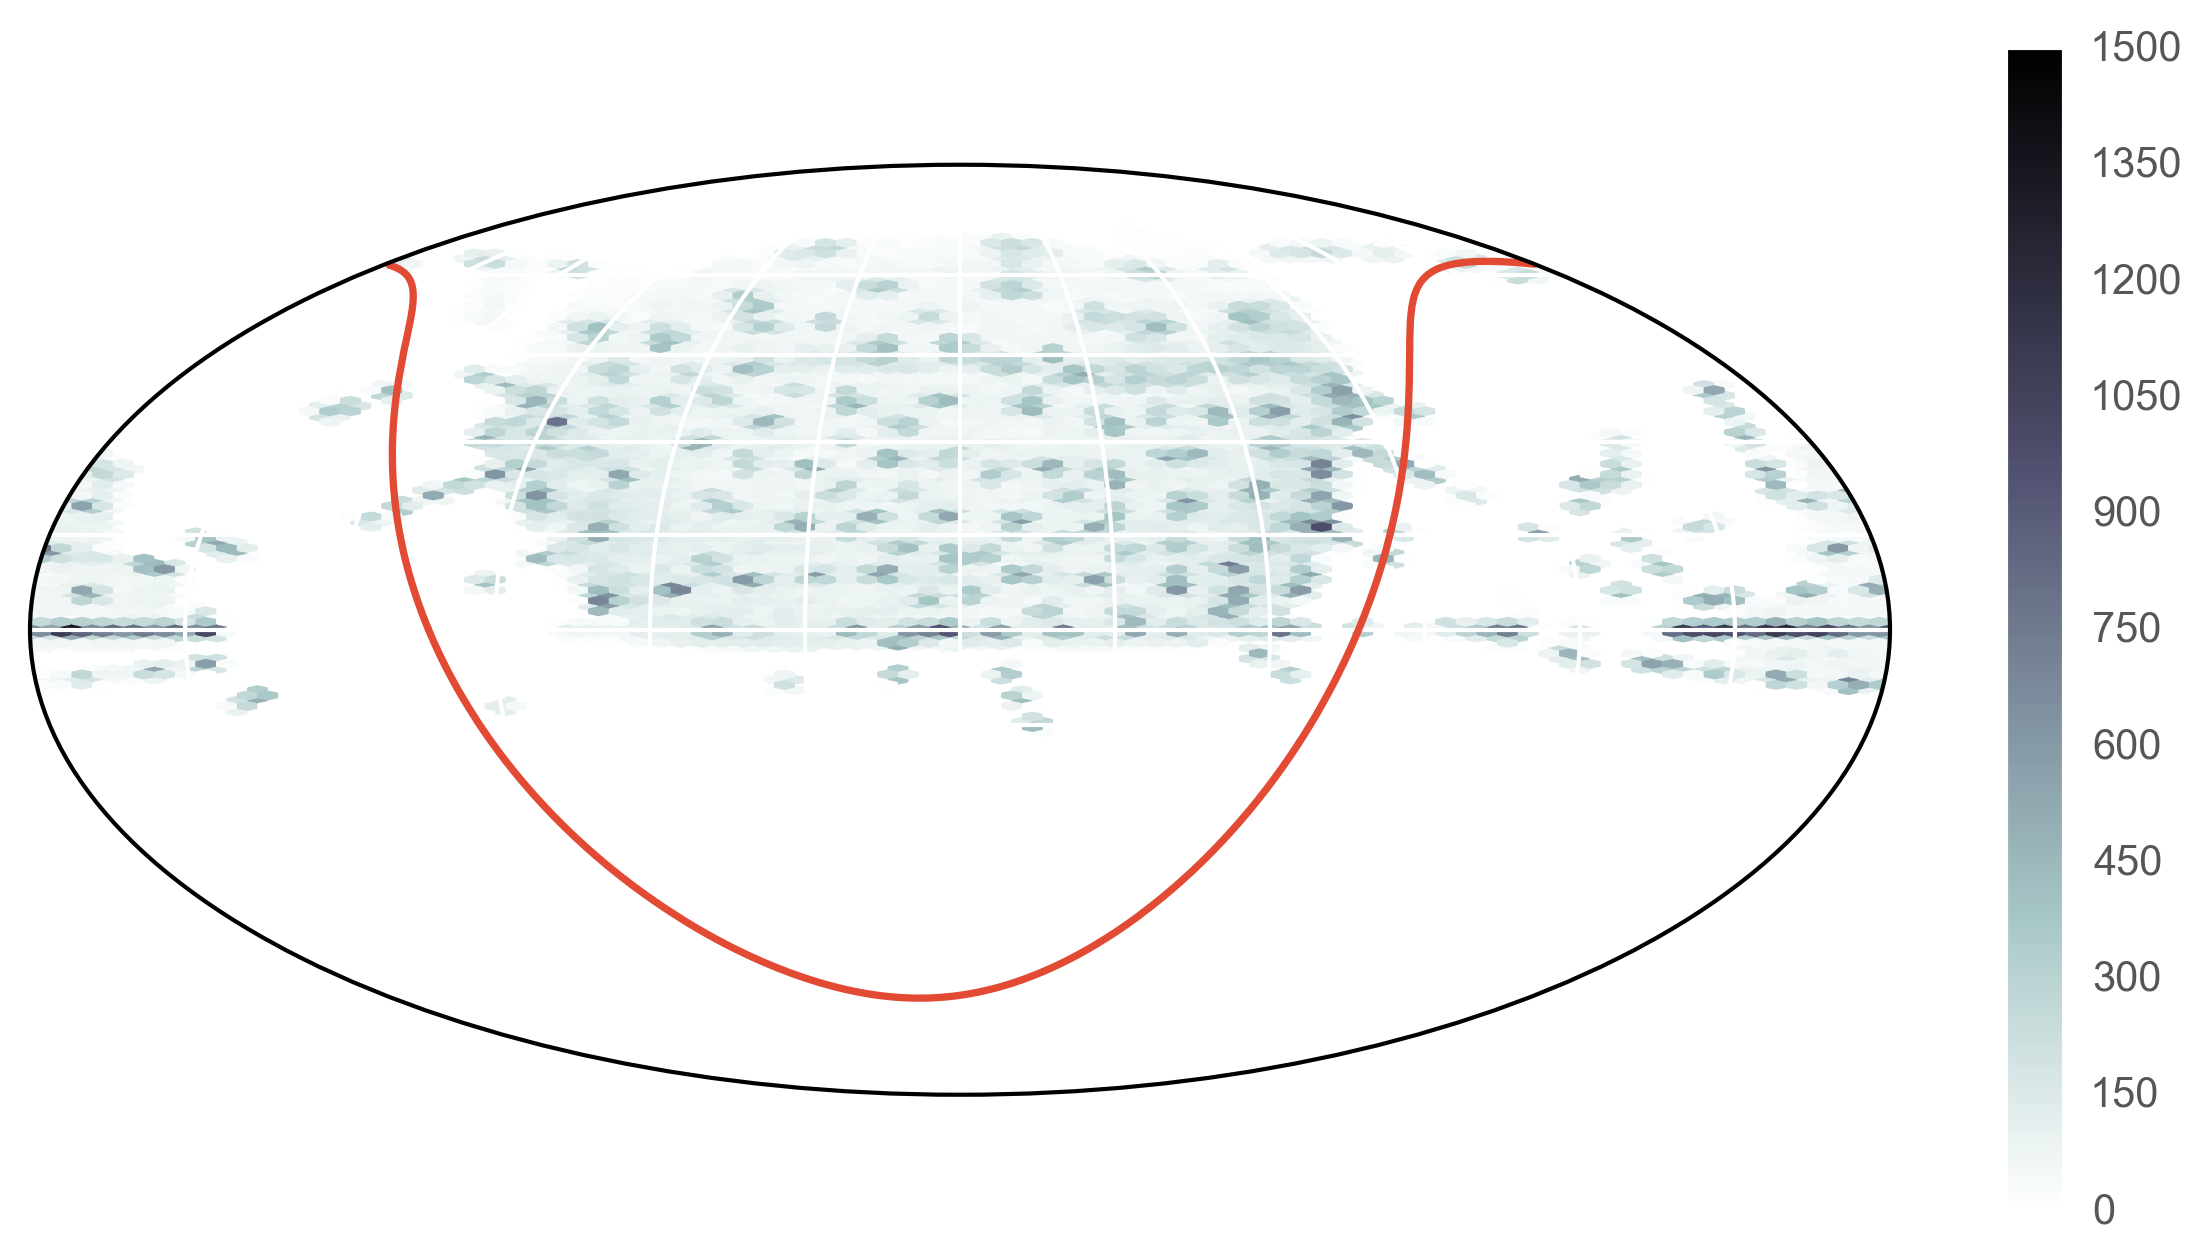
\includegraphics[width=0.73\linewidth]{figures/4_expt1/sdss_train_stars}
		\caption{The distribution of stars.}
		\label{fig:training_s}
	\end{subfigure}
	\begin{subfigure}{\textwidth}
		\centering
		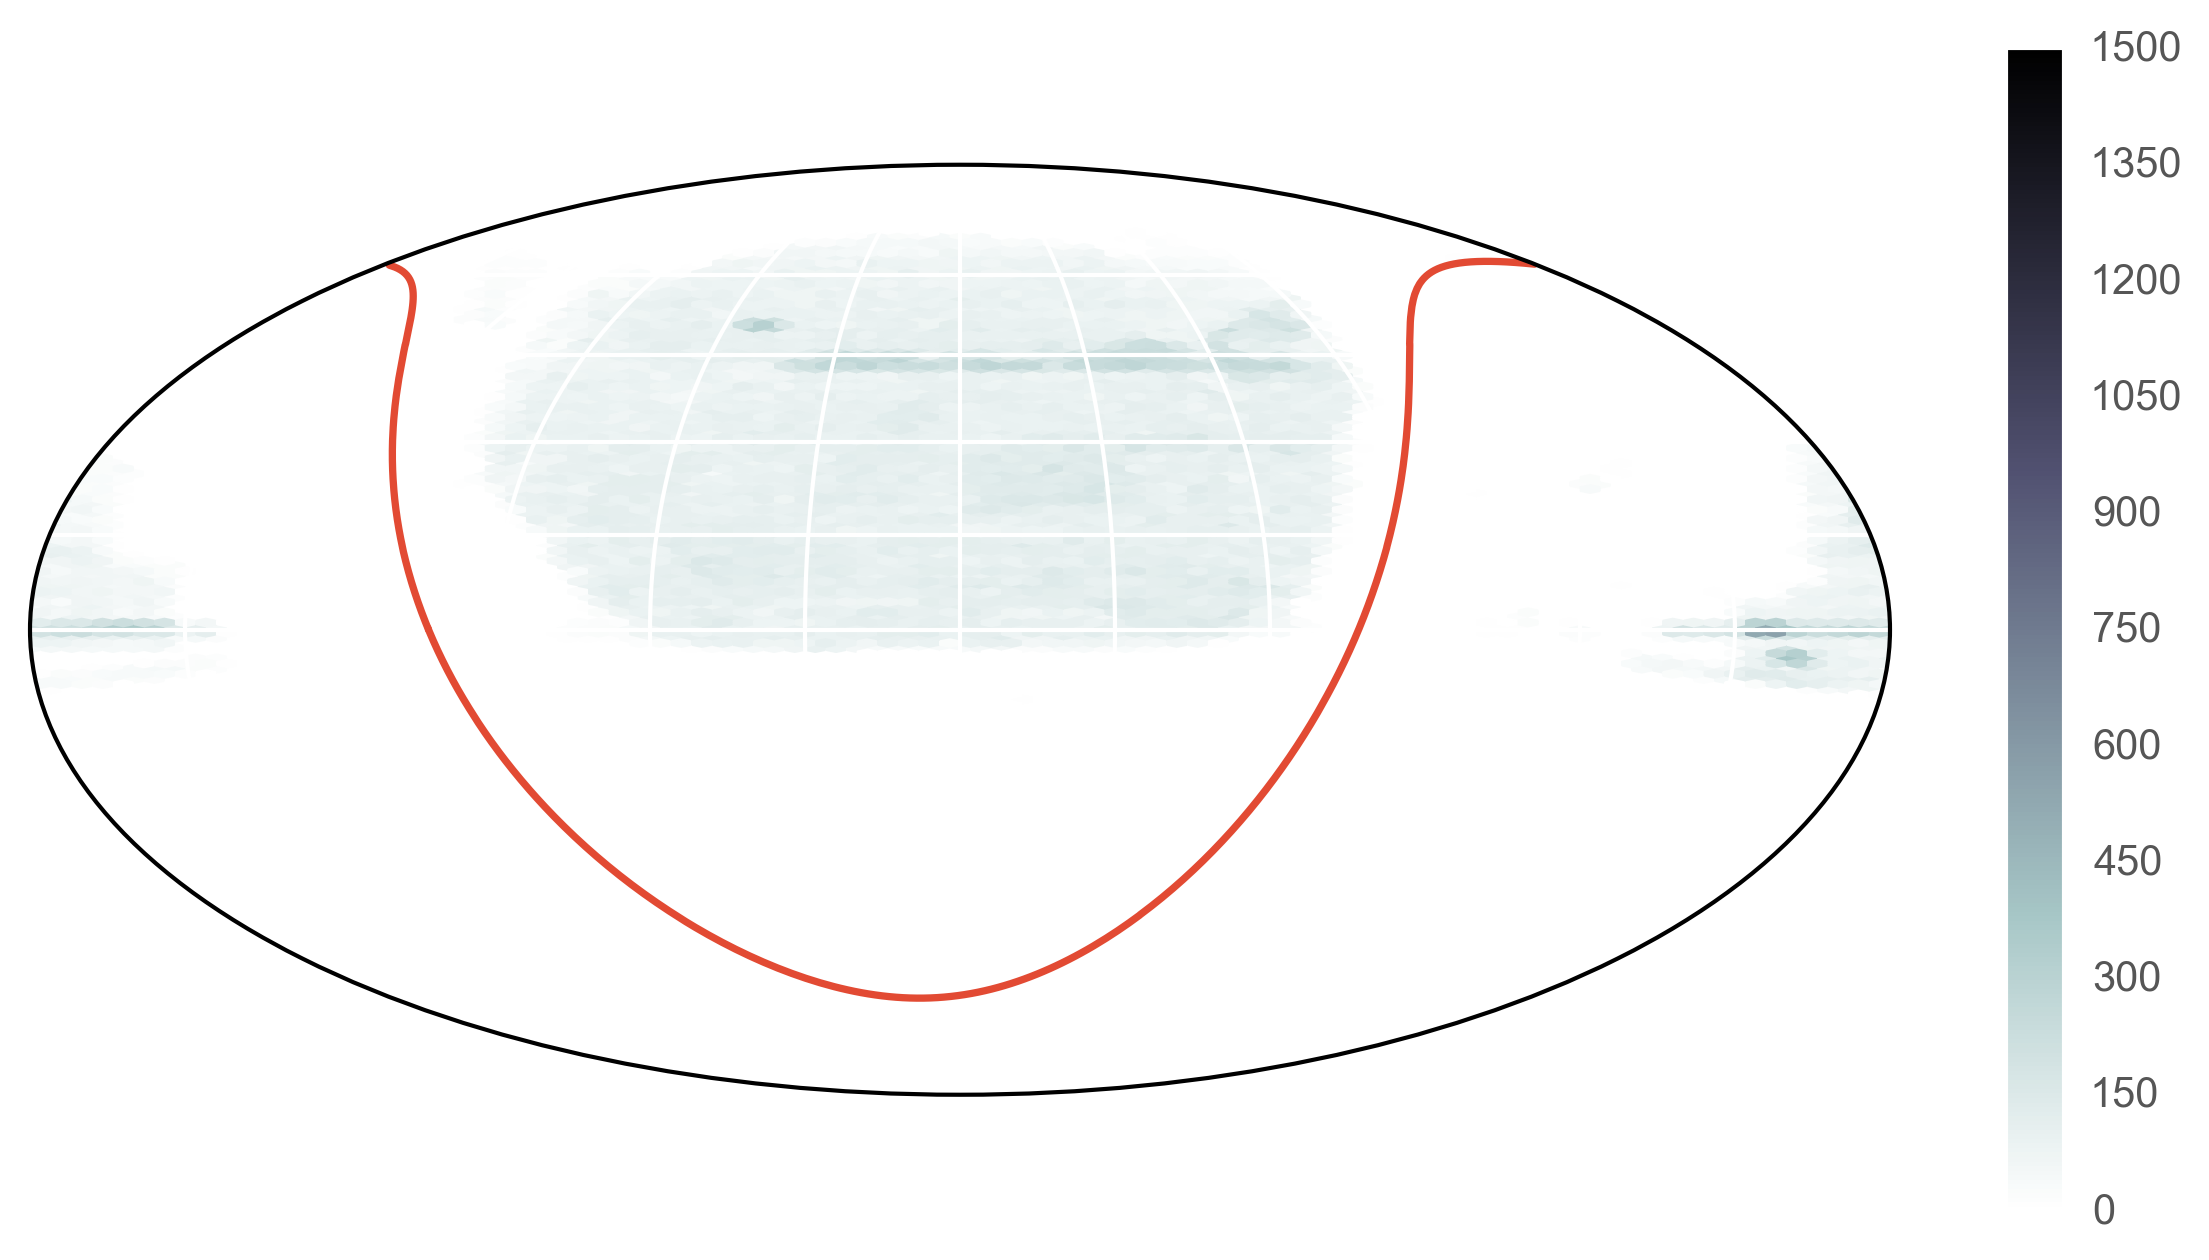
\includegraphics[width=0.73\linewidth]{figures/4_expt1/sdss_train_quasars}
		\caption{The distribution of quasars.}
		\label{fig:training_q}
	\end{subfigure}
	\caption[Distribution map of labelled objects in the SDSS]{The distribution map of
		the 2.8 million labelled objects in the SDSS: Observe that the
		galaxies are mostly uniformly distributed in the survey, while the stars are not.
		We also do not have a lot of examples of quasars.}
	\label{fig:training_dist}
\end{figure}

\begin{figure}[p]
	\centering
	\begin{subfigure}{\textwidth}
		\centering
		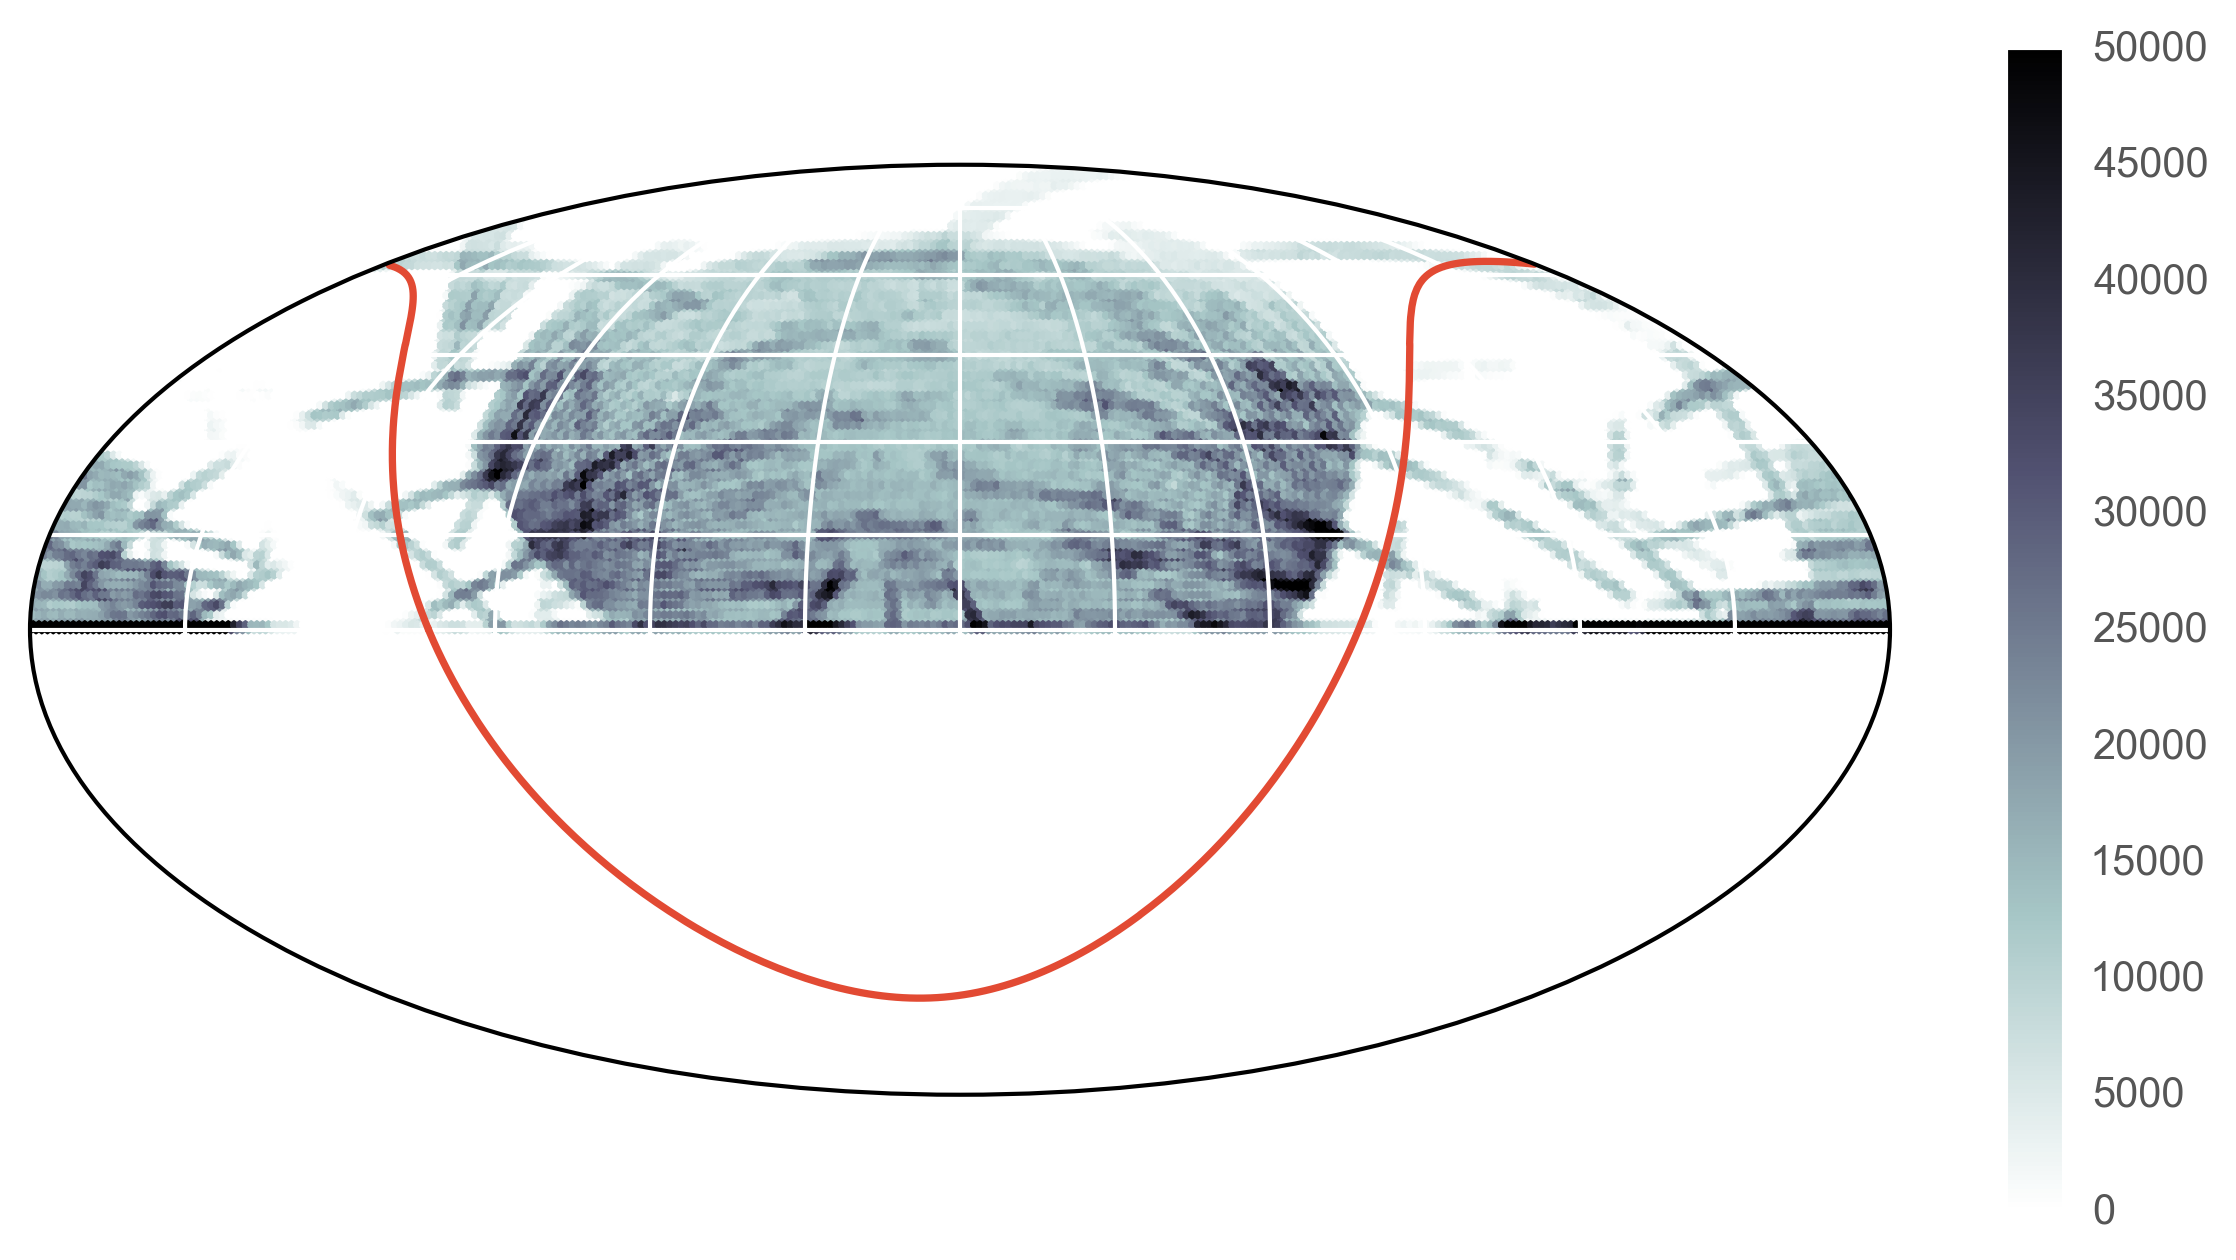
\includegraphics[width=0.75\textwidth]{figures/4_expt1/map_prediction_forest_galaxies}
		\caption{Distribution of galaxies.}
		\label{fig:random1}
	\end{subfigure}\\
	\begin{subfigure}{\textwidth}
		\centering
		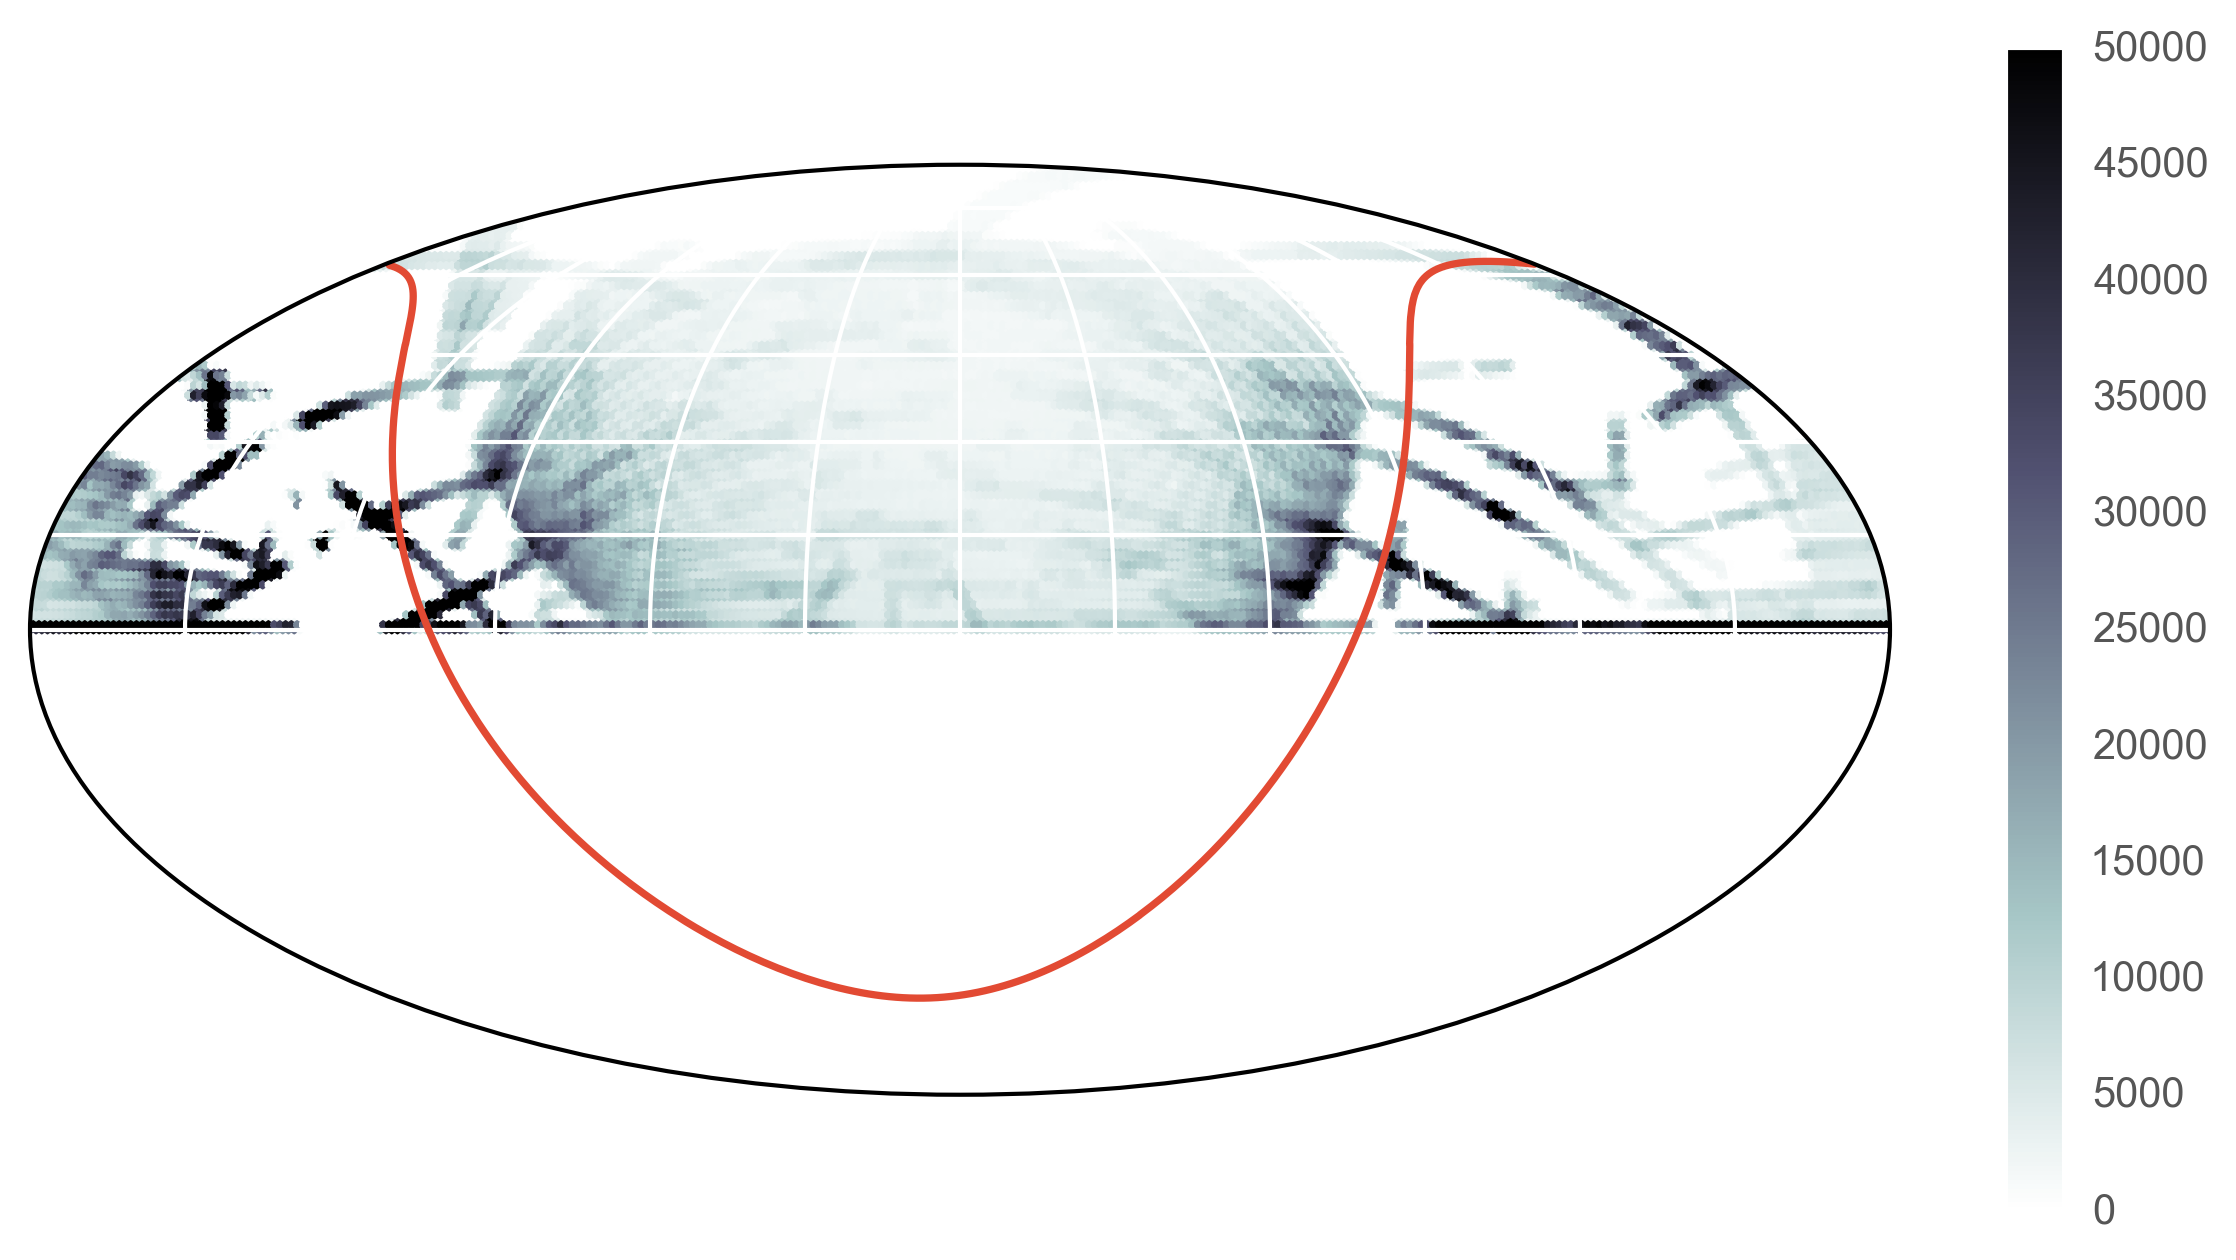
\includegraphics[width=0.75\linewidth]{figures/4_expt1/map_prediction_forest_stars}
		\caption{Distribution of stars.}
		\label{fig:random2}
	\end{subfigure}
	\begin{subfigure}{\textwidth}
		\centering
		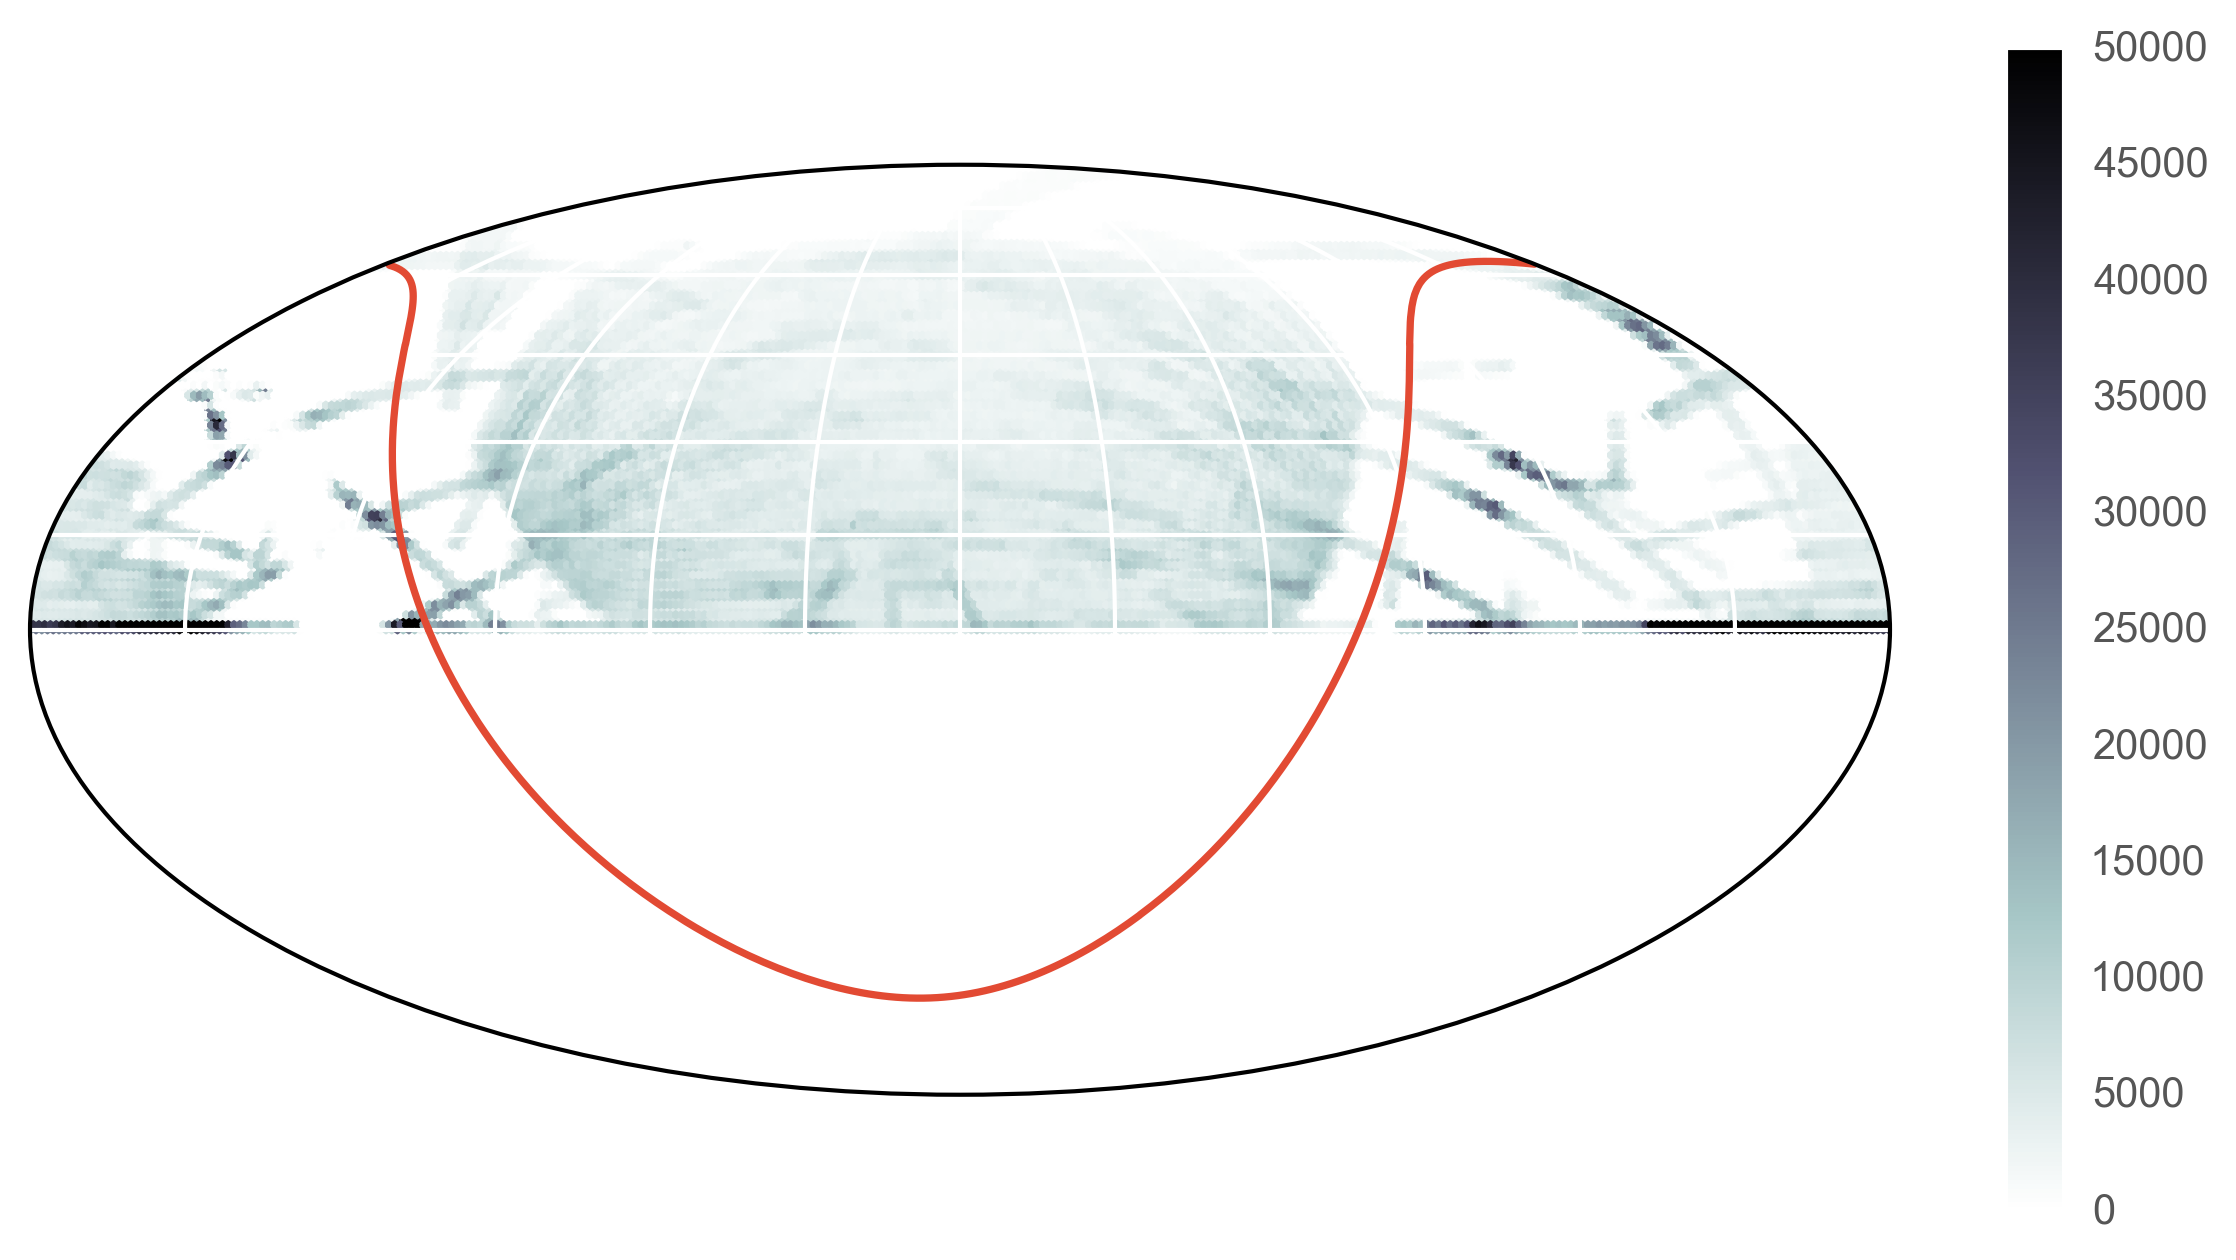
\includegraphics[width=0.75\linewidth]{figures/4_expt1/map_prediction_forest_quasars}
		\caption{Distribution of quasars.}
		\label{fig:random3}
	\end{subfigure}
	\caption[Map of predicted labels on all SDSS data.]{
		Map of predicted labels on the whole SDSS dataset using random forest: This
		map is, however, only moderately useful, since it is not a random sample of the sky.}
	\label{fig:forest}
\end{figure}


\begin{figure}[p]
	\centering
	\begin{subfigure}{\textwidth}
		\centering
		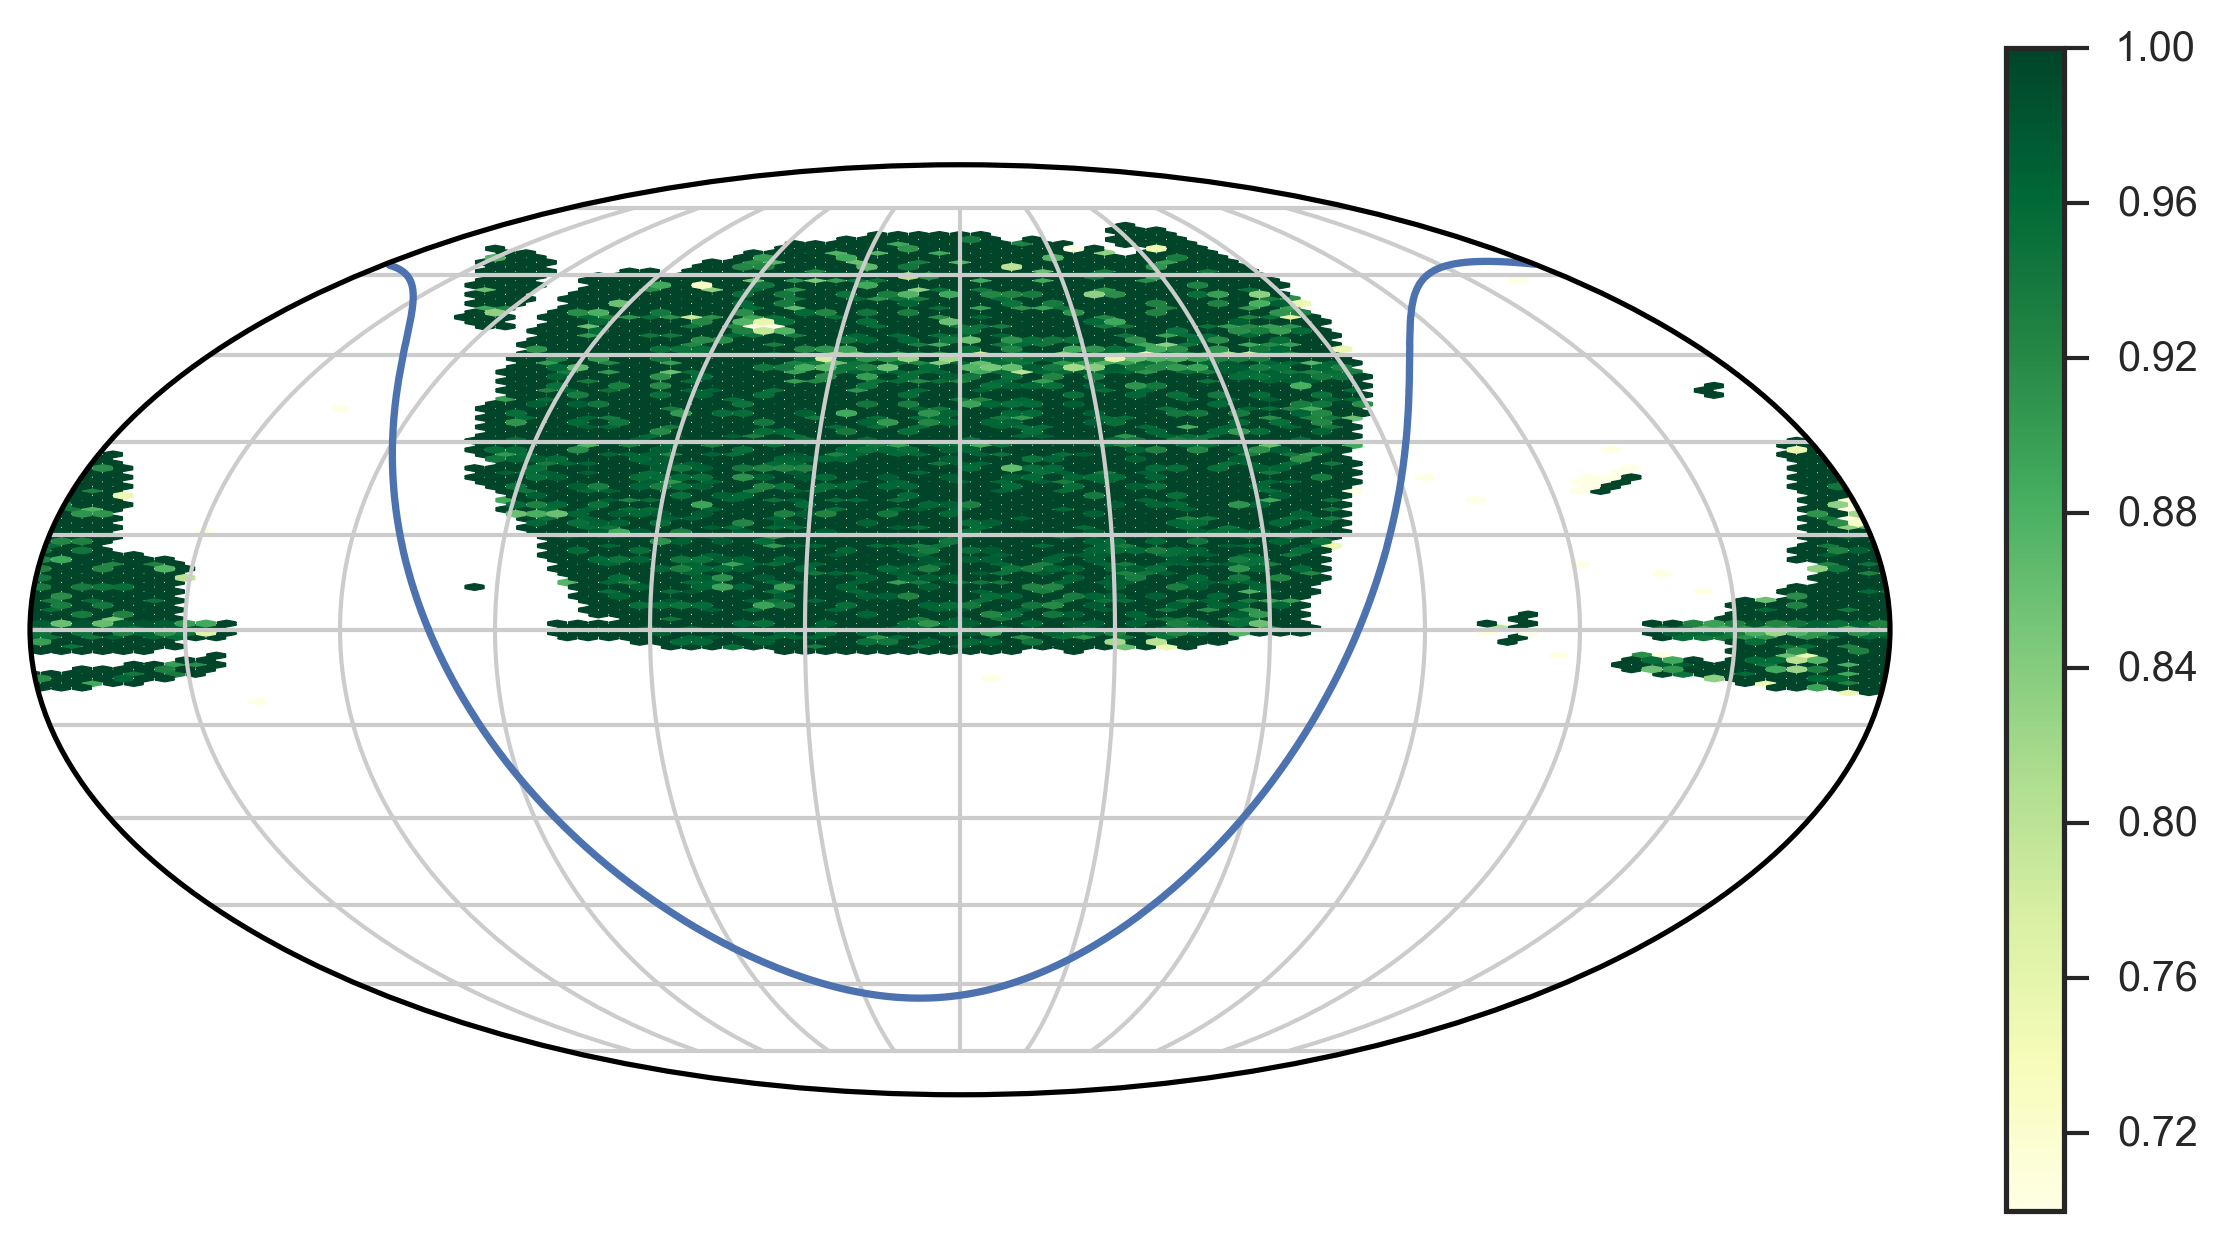
\includegraphics[width=0.75\textwidth]{figures/4_expt1/map_recall_forest_all_Galaxy}
		\caption{Recall of galaxies.}
		\label{fig:map_recall_forest_all_Galaxy}
	\end{subfigure}\\
	\begin{subfigure}{\textwidth}
		\centering
		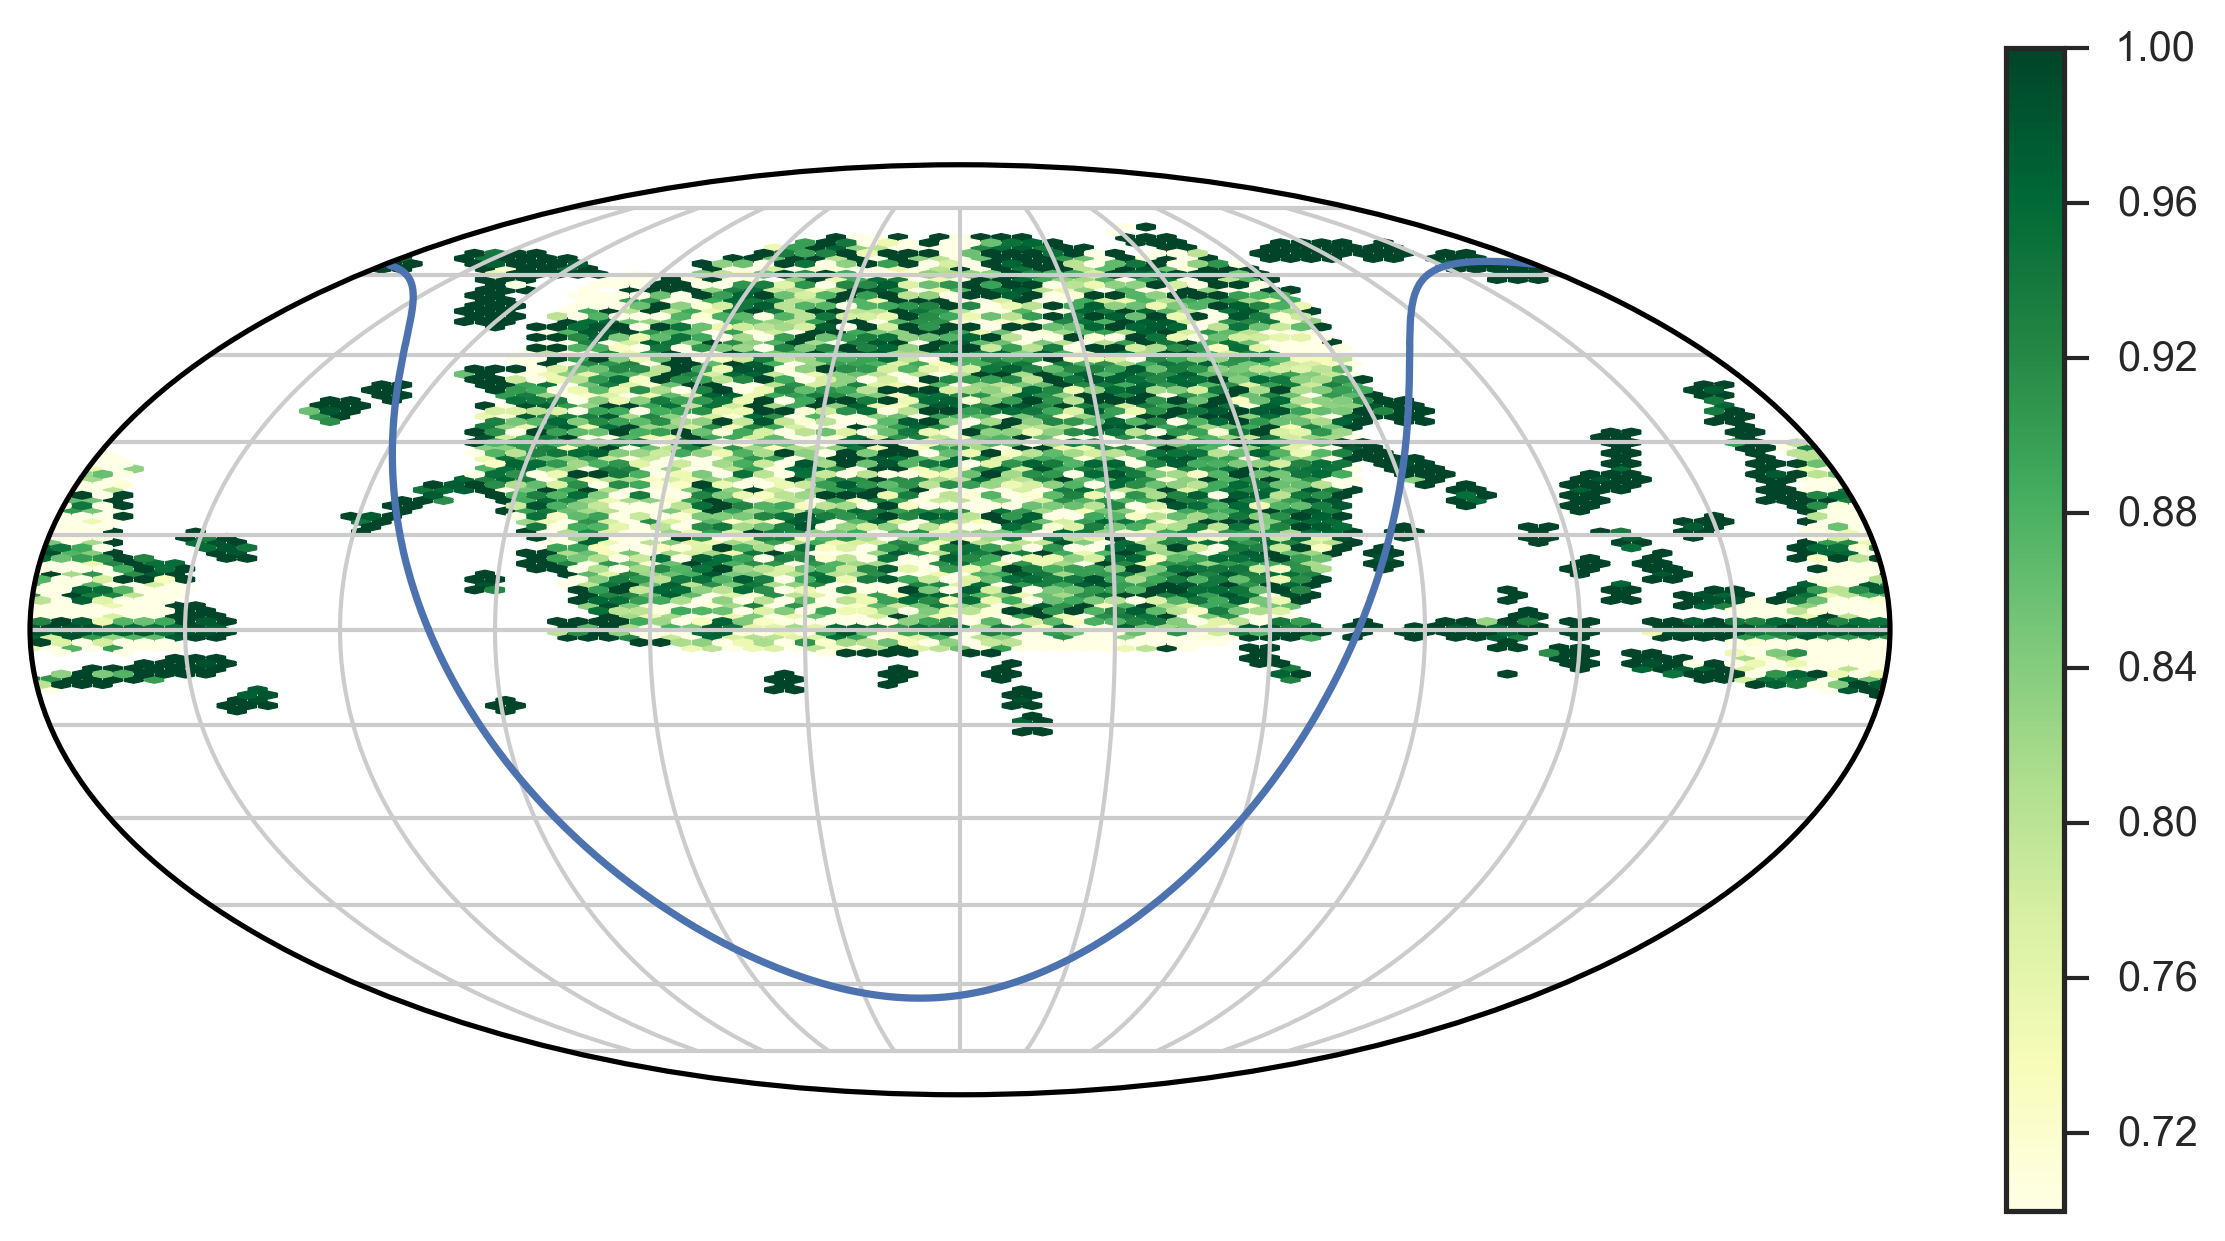
\includegraphics[width=0.75\linewidth]{figures/4_expt1/map_recall_forest_all_Star}
		\caption{Recall of stars.}
		\label{fig:map_recall_forest_all_Star}
	\end{subfigure}
	\begin{subfigure}{\textwidth}
		\centering
		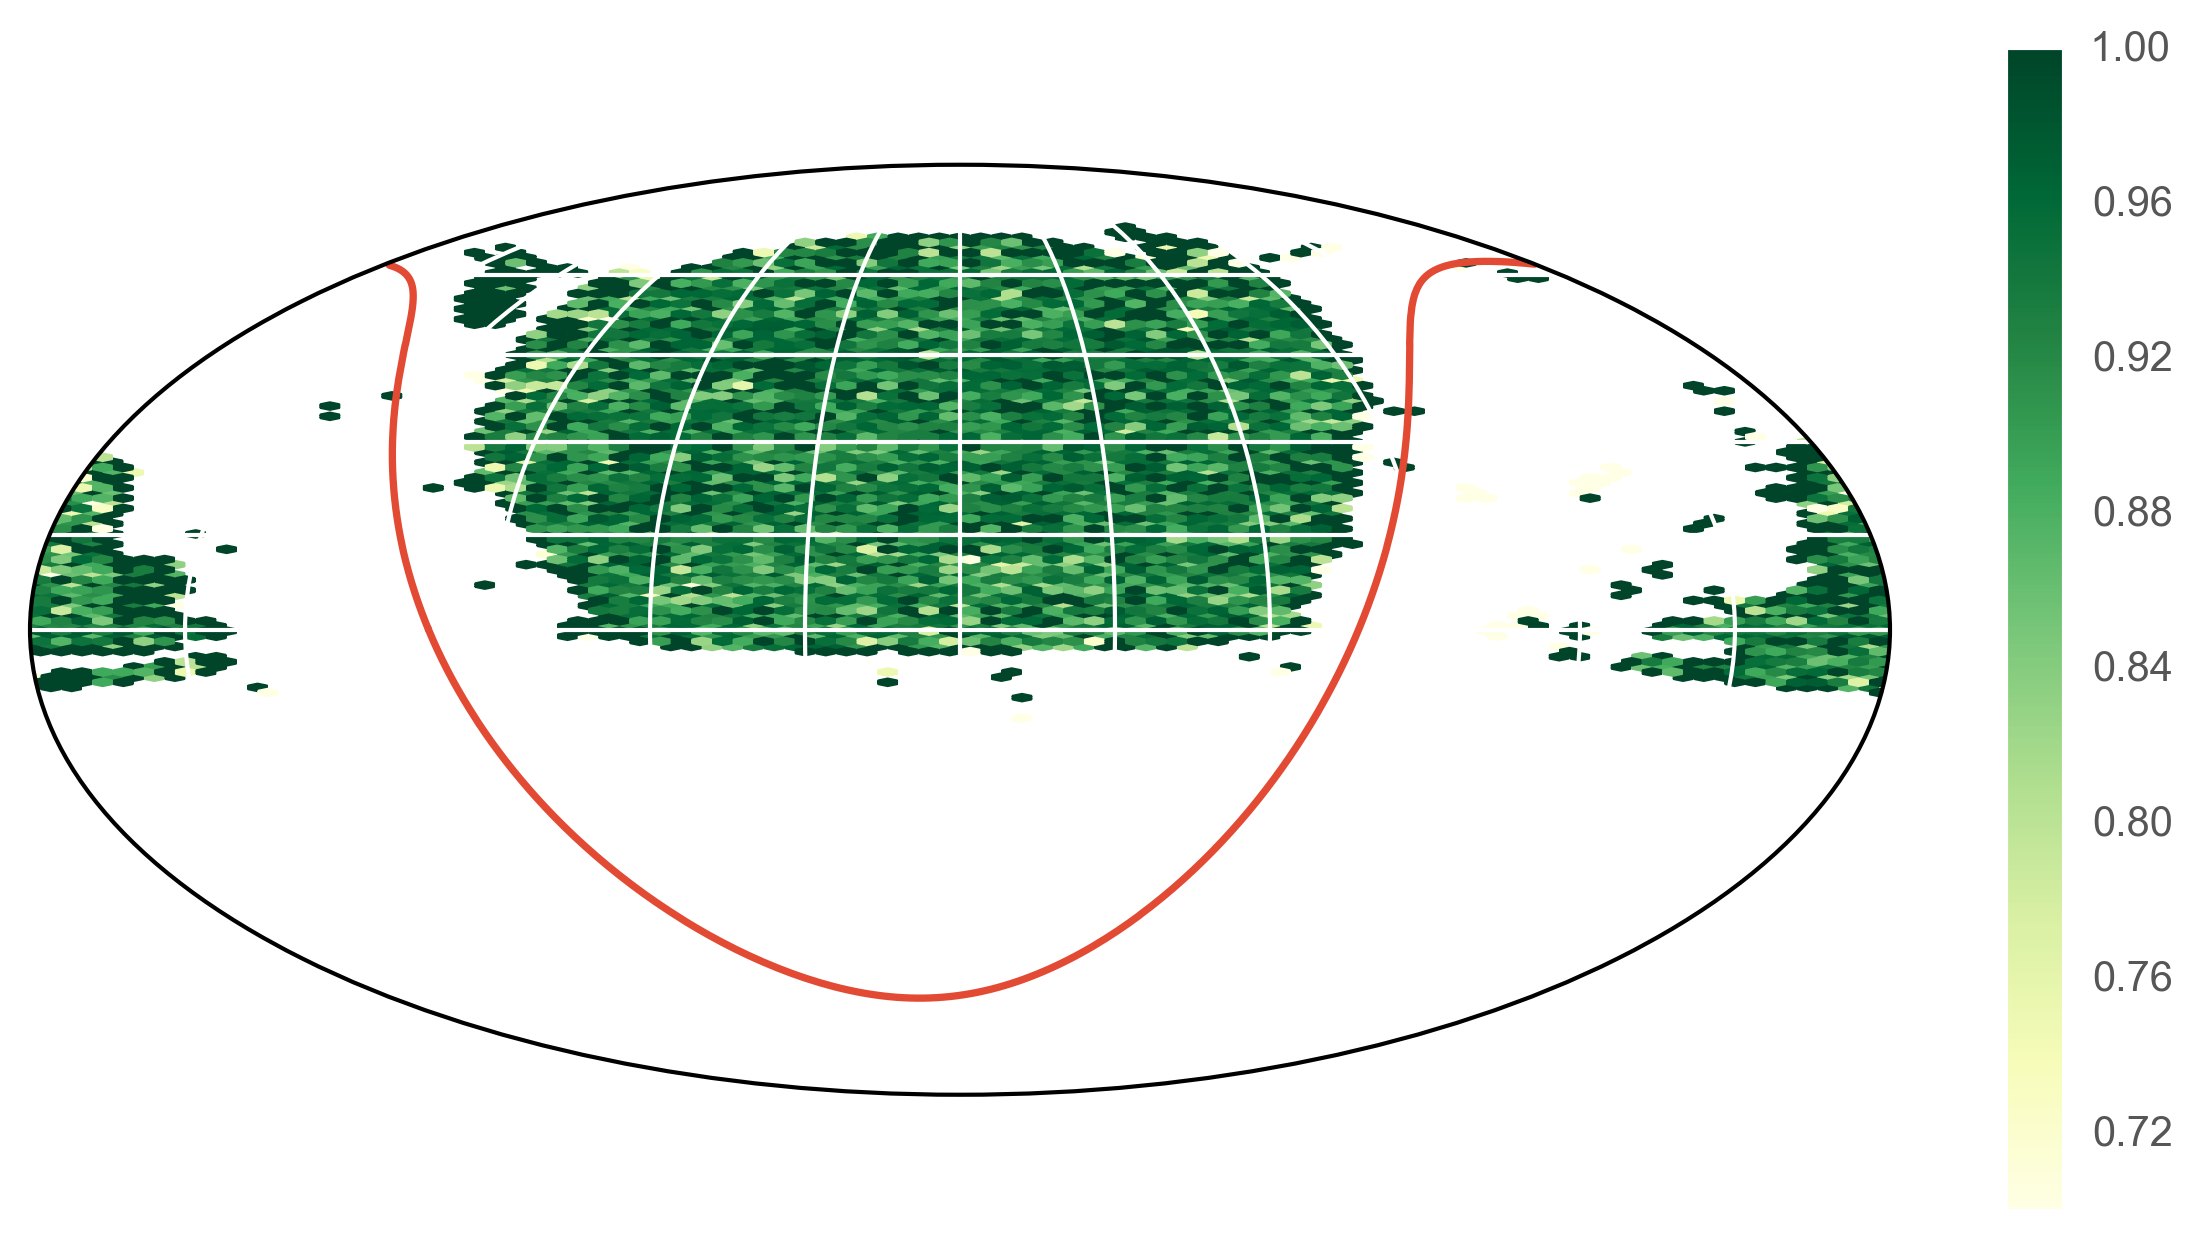
\includegraphics[width=0.75\linewidth]{figures/4_expt1/map_recall_forest_all_Quasar}
		\caption{Recall of quasars.}
		\label{fig:map_recall_forest_all_Quasar}
	\end{subfigure}
	\caption[Recall maps of the random forest]{Recall maps of the random forest: The recall of galaxies
        is almost perfect, while the recall of stars is fairly average.}
    
    \label{fig:map_recall_forest_all}
\end{figure}



%%% Local Variables: 
%%% mode: latex
%%% TeX-master: "thesis"
%%% End: 
